% Options for packages loaded elsewhere
\PassOptionsToPackage{unicode}{hyperref}
\PassOptionsToPackage{hyphens}{url}
\PassOptionsToPackage{dvipsnames,svgnames,x11names}{xcolor}
%
\documentclass[
]{article}

\usepackage{amsmath,amssymb}
\usepackage{iftex}
\ifPDFTeX
  \usepackage[T1]{fontenc}
  \usepackage[utf8]{inputenc}
  \usepackage{textcomp} % provide euro and other symbols
\else % if luatex or xetex
  \usepackage{unicode-math}
  \defaultfontfeatures{Scale=MatchLowercase}
  \defaultfontfeatures[\rmfamily]{Ligatures=TeX,Scale=1}
\fi
\usepackage[]{Times}
\ifPDFTeX\else  
    % xetex/luatex font selection
    \setmainfont[]{Latin Modern Roman}
  \setmathfont[]{Latin Modern Math}
\fi
% Use upquote if available, for straight quotes in verbatim environments
\IfFileExists{upquote.sty}{\usepackage{upquote}}{}
\IfFileExists{microtype.sty}{% use microtype if available
  \usepackage[]{microtype}
  \UseMicrotypeSet[protrusion]{basicmath} % disable protrusion for tt fonts
}{}
\makeatletter
\@ifundefined{KOMAClassName}{% if non-KOMA class
  \IfFileExists{parskip.sty}{%
    \usepackage{parskip}
  }{% else
    \setlength{\parindent}{0pt}
    \setlength{\parskip}{6pt plus 2pt minus 1pt}}
}{% if KOMA class
  \KOMAoptions{parskip=half}}
\makeatother
\usepackage{xcolor}
\setlength{\emergencystretch}{3em} % prevent overfull lines
\setcounter{secnumdepth}{5}
% Make \paragraph and \subparagraph free-standing
\makeatletter
\ifx\paragraph\undefined\else
  \let\oldparagraph\paragraph
  \renewcommand{\paragraph}{
    \@ifstar
      \xxxParagraphStar
      \xxxParagraphNoStar
  }
  \newcommand{\xxxParagraphStar}[1]{\oldparagraph*{#1}\mbox{}}
  \newcommand{\xxxParagraphNoStar}[1]{\oldparagraph{#1}\mbox{}}
\fi
\ifx\subparagraph\undefined\else
  \let\oldsubparagraph\subparagraph
  \renewcommand{\subparagraph}{
    \@ifstar
      \xxxSubParagraphStar
      \xxxSubParagraphNoStar
  }
  \newcommand{\xxxSubParagraphStar}[1]{\oldsubparagraph*{#1}\mbox{}}
  \newcommand{\xxxSubParagraphNoStar}[1]{\oldsubparagraph{#1}\mbox{}}
\fi
\makeatother


\providecommand{\tightlist}{%
  \setlength{\itemsep}{0pt}\setlength{\parskip}{0pt}}\usepackage{longtable,booktabs,array}
\usepackage{calc} % for calculating minipage widths
% Correct order of tables after \paragraph or \subparagraph
\usepackage{etoolbox}
\makeatletter
\patchcmd\longtable{\par}{\if@noskipsec\mbox{}\fi\par}{}{}
\makeatother
% Allow footnotes in longtable head/foot
\IfFileExists{footnotehyper.sty}{\usepackage{footnotehyper}}{\usepackage{footnote}}
\makesavenoteenv{longtable}
\usepackage{graphicx}
\makeatletter
\def\maxwidth{\ifdim\Gin@nat@width>\linewidth\linewidth\else\Gin@nat@width\fi}
\def\maxheight{\ifdim\Gin@nat@height>\textheight\textheight\else\Gin@nat@height\fi}
\makeatother
% Scale images if necessary, so that they will not overflow the page
% margins by default, and it is still possible to overwrite the defaults
% using explicit options in \includegraphics[width, height, ...]{}
\setkeys{Gin}{width=\maxwidth,height=\maxheight,keepaspectratio}
% Set default figure placement to htbp
\makeatletter
\def\fps@figure{htbp}
\makeatother
% definitions for citeproc citations
\NewDocumentCommand\citeproctext{}{}
\NewDocumentCommand\citeproc{mm}{%
  \begingroup\def\citeproctext{#2}\cite{#1}\endgroup}
\makeatletter
 % allow citations to break across lines
 \let\@cite@ofmt\@firstofone
 % avoid brackets around text for \cite:
 \def\@biblabel#1{}
 \def\@cite#1#2{{#1\if@tempswa , #2\fi}}
\makeatother
\newlength{\cslhangindent}
\setlength{\cslhangindent}{1.5em}
\newlength{\csllabelwidth}
\setlength{\csllabelwidth}{3em}
\newenvironment{CSLReferences}[2] % #1 hanging-indent, #2 entry-spacing
 {\begin{list}{}{%
  \setlength{\itemindent}{0pt}
  \setlength{\leftmargin}{0pt}
  \setlength{\parsep}{0pt}
  % turn on hanging indent if param 1 is 1
  \ifodd #1
   \setlength{\leftmargin}{\cslhangindent}
   \setlength{\itemindent}{-1\cslhangindent}
  \fi
  % set entry spacing
  \setlength{\itemsep}{#2\baselineskip}}}
 {\end{list}}
\usepackage{calc}
\newcommand{\CSLBlock}[1]{\hfill\break\parbox[t]{\linewidth}{\strut\ignorespaces#1\strut}}
\newcommand{\CSLLeftMargin}[1]{\parbox[t]{\csllabelwidth}{\strut#1\strut}}
\newcommand{\CSLRightInline}[1]{\parbox[t]{\linewidth - \csllabelwidth}{\strut#1\strut}}
\newcommand{\CSLIndent}[1]{\hspace{\cslhangindent}#1}

\usepackage{booktabs}
\usepackage{caption}
\usepackage{longtable}
\usepackage{colortbl}
\usepackage{array}
\usepackage{tipa}
\usepackage{booktabs}
\DeclareTextFontCommand\textphonetic{\ipafont}
\usepackage[utf8]{inputenc}
\usepackage{CJKutf8}
\usepackage{arxiv}
\usepackage{orcidlink}
\usepackage{amsmath}
\usepackage[T1]{fontenc}
\makeatletter
\@ifpackageloaded{caption}{}{\usepackage{caption}}
\AtBeginDocument{%
\ifdefined\contentsname
  \renewcommand*\contentsname{Table of contents}
\else
  \newcommand\contentsname{Table of contents}
\fi
\ifdefined\listfigurename
  \renewcommand*\listfigurename{List of Figures}
\else
  \newcommand\listfigurename{List of Figures}
\fi
\ifdefined\listtablename
  \renewcommand*\listtablename{List of Tables}
\else
  \newcommand\listtablename{List of Tables}
\fi
\ifdefined\figurename
  \renewcommand*\figurename{Figure}
\else
  \newcommand\figurename{Figure}
\fi
\ifdefined\tablename
  \renewcommand*\tablename{Table}
\else
  \newcommand\tablename{Table}
\fi
}
\@ifpackageloaded{float}{}{\usepackage{float}}
\floatstyle{ruled}
\@ifundefined{c@chapter}{\newfloat{codelisting}{h}{lop}}{\newfloat{codelisting}{h}{lop}[chapter]}
\floatname{codelisting}{Listing}
\newcommand*\listoflistings{\listof{codelisting}{List of Listings}}
\makeatother
\makeatletter
\makeatother
\makeatletter
\@ifpackageloaded{caption}{}{\usepackage{caption}}
\@ifpackageloaded{subcaption}{}{\usepackage{subcaption}}
\makeatother
\ifLuaTeX
\usepackage[bidi=basic]{babel}
\else
\usepackage[bidi=default]{babel}
\fi
\babelprovide[main,import]{english}
\ifPDFTeX
\else
\babelfont{rm}[]{Latin Modern Roman}
\fi
% get rid of language-specific shorthands (see #6817):
\let\LanguageShortHands\languageshorthands
\def\languageshorthands#1{}
\ifLuaTeX
  \usepackage{selnolig}  % disable illegal ligatures
\fi
\usepackage{bookmark}

\IfFileExists{xurl.sty}{\usepackage{xurl}}{} % add URL line breaks if available
\urlstyle{same} % disable monospaced font for URLs
\hypersetup{
  pdftitle={The role of cognateness in native spoken word recognition},
  pdfauthor={Gonzalo Garcia-Castro; Serene Siow; Kim Plunkett; Nuria Sebastian-Galles},
  pdflang={en},
  pdfkeywords={cognate, spoken word
recognition, phonology, bilingualism, non-native speech
processing, lexical access},
  colorlinks=true,
  linkcolor={blue},
  filecolor={Maroon},
  citecolor={Blue},
  urlcolor={Blue},
  pdfcreator={LaTeX via pandoc}}

\usepackage{lineno}
\linenumbers
\newcommand{\runninghead}{A Preprint }
\renewcommand{\runninghead}{Cognateness and recognition of foreign
words }
\title{The role of cognateness in native spoken word recognition}
\author{\textbf{Gonzalo
Garcia-Castro}~\orcidlink{0000-0002-8553-4209}\\Center for Brain and
Cognition\\Universitat Pompeu Fabra\\Barcelona,
08005\\\texttt{\href{mailto:gonzalo.garciadecastro@upf.edu}{gonzalo.garciadecastro@upf.edu}}\And\textbf{Serene
Siow}~\orcidlink{0000-0001-6482-2191}\\Department of Experimental
Psychology\\University of Oxford\\Oxford, OX2
6GG\\\texttt{\href{mailto:siow.serene@gmail.com}{siow.serene@gmail.com}}\And\textbf{Kim
Plunkett}~\orcidlink{0000-0003-0216-7480}\\Department of Experimental
Psychology\\University of Oxford\\Oxford, OX2
6GG\\\texttt{\href{mailto:kim.plunkett@psy.ox.ac.uk}{kim.plunkett@psy.ox.ac.uk}}\And\textbf{Nuria
Sebastian-Galles}~\orcidlink{0000-0001-6938-2498}\\Center for Brain and
Cognition\\Universitat Pompeu Fabra\\Barcelona,
08005\\\texttt{\href{mailto:nuria.sebastian@upf.edu}{nuria.sebastian@upf.edu}}}
\date{}
\begin{document}
\maketitle
{\bfseries \emph Keywords}
\def\sep{\textbullet\ }
cognate \sep spoken word
recognition \sep phonology \sep bilingualism \sep non-native speech
processing \sep 
lexical access


\section{Introduction}\label{introduction}

When some German speakers listened to the song \emph{The Power} by SNAP!
(\emph{Coyote Ugly}, 2000), many of them misheard the line ``I've got
the power'' as \emph{Agatha Bauer!} When Michael Jackson vocalised
``ma-ma-coo-sah'' in his song \emph{Wanna Be Startin' Somethin'}
(\emph{Thriller}, 1982), some Dutch speakers understood \emph{mama
appelsap} {[}mama applejuice{]}. When Spanish speakers listen to the
line ``Circumvent your thick ego'' from the song \emph{Pictures} by
System of a Down (\emph{Steal this Album!}, 2002), they tend to hear
\emph{Sácame de aquí, King-Kong} {[}take me out of here, King-Kong{]}.
When Japanese speakers listen to the line ``I want to hold your hand''
in the homonym song by The Beatles (\emph{Meet The Beatles}, 1964), they
often mishear \emph{Aho na hōnyōhan} {[}stupid urinator{]}. Outrageous
as these examples might sound to speakers of other languages, many
readers may know a few cases in their own native language. This auditory
illusion can feel quite real, and often inevitable after the first time
it happens. In Japanese, this phenomenon takes the name \emph{Soramimi}
(lit. ``empty ear''), after the \emph{Soramimi Hour}---a section of the
program \emph{Tamori Club} hosted by comedian Morita Kazuyoshi
(Tamori)---in which instances of this illusion were presented with
comedy purposes. Soramimi is a particular case of \emph{homophonic
translation}: words or phrases in one language are translated into
similar-sounding words and phrases in a different language, without
necessarily preserving the meaning. This phenomenon extends beyond song
lyrics, and may occur anytime when listening to non-native speech. For
instance, when listening to ``You know me?'' (\textipa{/ju: n@U mi:}/)
in English, Japanese-native listeners tend to understand \emph{yunomi}
(/\textipa{jUnomi}/), which is a type of Japanese teacup. Overall, the
occurence of Soramimi---and more generally, homophonic
translations---suggests that speech in an unfamiliar language has the
potential to activate lexical representations in the native language.

Although homophonic translations do not necessarily take place with the
preservation of meaning---which often results in outrageous
mistranslations like the ones aforementioned---homophonic translations
sometimes may lead to the activation of the intended meaning (i.e., a
correct translation). For example, imagine a Spanish native with no
previous familiarity with any other language listening to French for the
first time. This listener may encounter the word /\textipa{"pOKt}/
(\emph{porte}), translation of door in French. When comparing the
phonemic transcription of the French to that of its Spanish translation
/\textipa{"pweR.ta}/ (\emph{puerta}), one may be led to infer that these
two words do not have much overlap. But one thing to note is that the
voiced uvular fricative consonant /\textipa{K}/ and the open-mid back
rounded vowel /\textipa{O}/, which do not exist in Spanish as phonemic
categories, can be perceived as allophonic variations the native
(Spanish) phonemes /\textipa{R}/ and /o/, as described by assimilation
models of phoneme perception (\citeproc{ref-best1988examination}{Best et
al., 1988}, \citeproc{ref-best2001discrimination}{2001}). Although this
phonetic mismatch between the non-native word and its translation can
have a noticeable toll on comprehension Cutler et al.
(\citeproc{ref-cutler2004patterns}{2004}), the Spanish listener may
still be able to activate the phonological representation of
/\textipa{"pweR.ta}/ (\emph{puerta}) from hearing the word-form
/\textipa{"pOKt}/ (\emph{porte}), ultimately allowing them to access the
correct semantic representation. Given enough phonological similarity
between the non-native word and its translation in the native language,
a naïve listener may succeed at word comprehension when listening to an
unfamiliar language. Such phonological similarity between translation
equivalents---known as \emph{cognateness}---is common across many
languages, and is often due to typological closeness and/or
socio-historical events involving the speakers of these languages (e.g.,
migration, social contact). For example, Romance languages such as
Spanish and Catalan share many form-similar translation equivalents
(\citeproc{ref-schepens2012distributions}{Schepens et al., 2012}), as in
the case of \emph{puerta} and \emph{porta} (\emph{door} in Spanish and
Catalan, respectively). Given no prior knowledge of either language, a
Spanish native speaker is likely to be much more successful at correctly
translating Catalan \emph{porta} than English \emph{door}, due to the
phonological and orthographic similarity of the former to the equivalent
in their native language.

While Soramimi, and more generally homophonic translation, are popular
and frequent phenomena, the psycholinguistic literature on the topic is
relatively scarce, and has mostly focused on the phonological variables
involved in the occurence of Soramimi. For instance, Otake
(\citeproc{ref-otake2007interlingual}{2007}) analysed 194 instances of
Soramimi, broadcasted between 1992 and 2007 by the TV show Soramimi
hour. These instances consisted of homophonic translations of English
song lyrics to Japanese words and phrases. The vast majority of the
reported instances were phrases (96\%) and a few, to single words (4\%).
The phonetic features of the presented English lyrics were preserved
with relatively high variability, with some Japanese resulting words or
phrases sharing high overlap with the original English strings of
sounds, and some sharing very little overlap. When analysing the few
instances of homophonic translations of single words, the author
identified three phonological processes that might explain how Japanese
listeners reconstructed the English input to generate the Japanese
words: insertion (e.g., \emph{cry} /\textipa{kraI}/ to \emph{kurai},
/\textipa{kuRai}/ {[}dark{]}), deletion (e.g., \emph{go},
/\textipa{goU}/ to \emph{go}, /go/ {[}go{]}, and alternation (e.g.,
\emph{low}, /\textipa{loU}/ to \emph{rou}, /\textipa{Roo}/ {[}wax{]}).
This suggests that the reported homophonic translations can be
explained, to some extent, as the result of the Japanese listeners
accommodating the strings of English sounds to the Japanese phoneme
inventory and Japanese phonotactics
(\citeproc{ref-dupoux1999epenthetic}{Dupoux et al., 1999};
\citeproc{ref-peperkamp2008perceptual}{Peperkamp et al., 2008}). Native
prosody also constrains the occurence of homophonic translations. For
instance, Kentner (\citeproc{ref-kentner2015rhythmic}{2015}) presented
in the auditory modality French-native and German-native participants
with English songs with lyrics. Homophonic translations followed
language-specific segmentation strategies. Most homophonic translations
reported by German-native participants resulted from inserting phrase
and word boundaries \emph{before} stressed syllables (following the more
frequent trochaic patter in German). On the contrary, most homophonic
translations reported by French-native participants resulted from
inserting phrase and word boundaries \emph{after} stressed syllables,
following the more frequent iambic pattern in French.

While the previous studies have address the phonological aspects of
homophonic translation, little attention has been paid to the dynamics
of lexical activation and competition that underlay this phenomenon. In
the present work we investigated the interplay between phonological
similarity and phonological neighbourhood density to examine how
listeners of an unfamiliar language activate lexical representations in
their native language. In particular, we studied how the presence of
phonological neighbours in the native language lexicon affects the
extent to which listeners are able to activate the correct translation
of an auditorily presented word in an unfamiliar language. We used a
translation elicitation task in which participants listened to words
from an unfamiliar language, and then tried to guess their translation
in their native language. We will henceforth refer to the
auditory-presented words heard by participants on each trial as
presented words, and the correct translation for the presented words as
target translations. We explored listeners' reliance on phonological
similarity to succeed in the task by manipulating the amount of
phonological similarity between the presented words and their target
translations. Since participants were unfamiliar with the presented
language, they could only use phonological similarity between the
presented language and their native language to successfully translate
the words. We therefore predicted that participants' performance should
increase when the translation pairs are phonologically more similar. We
also predicted that there is a minimum threshold of phonological
similarity to be sufficient for translation.

We further investigated the effect of phonological competitors. Even if
the presented word and its target translation share high phonological
similarity, participants may still provide incorrect translations if the
presented word also shares high phonological similarity with other words
in the native language. Words with denser phonological neighbourhoods
are recognised more slowly and less accurately than words with sparser
phonological neighbourhoods (\citeproc{ref-dufour2003lexical}{Dufour \&
Peereman, 2003}; \citeproc{ref-goldinger1989priming}{Goldinger et al.,
1989}; \citeproc{ref-hamburger1996phonological}{Hamburger \& Slowiaczek,
1996}; \citeproc{ref-luce1990similarity}{Luce et al., 1990};
\citeproc{ref-luce1998recognizing}{Luce \& Pisoni, 1998}). This is
especially true if such neighbours share higher phonological similarity
with the presented word, or are lexically more frequent than the target
translation (\citeproc{ref-luce1998recognizing}{Luce \& Pisoni, 1998}).
Since the interference effects of phonological neighbourhood density has
also been reported across languages
(\citeproc{ref-weber2004lexical}{Weber \& Cutler, 2004}), we
hypothesised that the size of the facilitatory role of phonological
similarity would be inversely proportional to the amount of
higher-frequency phonological neighbours of the presented word in the
target language. In the case of non-native speech recognition, the
presence of cross-linguistic pairs which are phonologically similar but
differ in meaning (e.g., false friends) may act as distractors during
lexical access, obstructing the selection of the appropriate target
translation in the listener's lexicon. For instance, Otwinowska \&
Szewczyk (\citeproc{ref-otwinowska2019more}{2019}) reported that false
friends were disadvantaged relative to non-cognates by Polish second
language learners, in contrast to cognates which were known better. It
is therefore important to investigate the joint effect of both cognates
and false friends when investigating the effect cross-linguistic
phonological similarity has on word recognition in a foreign language.
This could shed light on available strategies and challenges associated
with the early stages of second language acquisition. For instance, one
could expect English participants to incorrectly translate the Spanish
word \emph{botón} as \emph{bottom} instead of as its correct translation
\emph{button}, due to combined effect of the close phonological
similarity between \emph{botón} and \emph{bottom} along with the high
lexical frequency of \emph{bottom} relative to \emph{button}. To test
this prediction, we developed a lexical frequency-dependent measure of
cross-language phonological neighbourhood density, in which a neighbour
is counted only if it is higher frequency and is one phoneme apart from
the presented word. If the phonological neighbourhood density of the
target translation affects participants' performance negatively, this
would suggest that competitors in the native language affect recognition
of non-native words during recognition of foreign speech. We conducted a
series of three experiments to test these predictions.

In Experiment 1, we collected data from two groups of British English
natives living in the United Kingdom. One group was presented with
Catalan words, the other with Spanish words. We examined the extent to
which participants were able to use the phonological similarity between
the presented word (in Catalan or Spanish) and its target translation to
provide accurate responses. In Experiment 2, we tested a group of
(European) Spanish natives in the same task, who were presented with
Catalan words. Catalan and Spanish are both Romance languages whose
close typological distance is reflected in the fact that they share many
cognates, where English is a Germanic language that shares considerably
fewer cognates with Catalan and Spanish. By testing participants
translating words from typologically close or distant languages, we
expected to widen the range of the phonological similarity scores of the
translation pairs involved in the experimental task, therefore allowing
us to explore potential cross-language differences in participant's
performance. One unexpected finding was that participants in Experiments
1 and 2 were surprisingly good at translating a subset of words which
had low phonological similarity with their correct translation. We were
concerned that this may be caused by some prior knowledge of specific
words by our participants, as some Spanish words are commonly seen in
media or product labels, making them familiar even to monolingual
speakers of English. In Experiment 3, we collected additional data from
a new group of British English natives. The design was closely modelled
after Experiment 1, except that after providing their response in each
trial, participants reported whether they had previous knowledge of the
presented word. In the final section of this paper, we present analyses
on the joint data sets of Experiments 1 to 3.

\section{Experiment 1}\label{experiment-1}

\subsection{Methods}\label{methods}

All materials, data, and code used in this study are hosted in the Open
Science Framework
\href{https://osf.io/9fjxm/?view_only=aab7636ce1af48cf832596a7ea9101c5/}{https://osf.io/9fjxm/}
and a GitHub repository
\url{https://github.com/gongcastro/translation-elicitation.git}, along
with additional notes.

\subsubsection{Participants}\label{participants}

Participants were recruited via Prolific (5£ compensation) and SONA
(compensation in academic credits), and gave informed consent before
providing any data and the study was conducted in accordance with
ethical standards of the Declaration of Helsinki and the protocol was by
the University of Oxford Medical Sciences Inter-Divisional Research
Ethics Committee (IDREC) (R60939/RE007). Participants were asked to
complete the experiment using a laptop in a quiet place with good
internet connection. Data collection took place from June 04th, 2020 to
June 25th, 2020. We collected data from 71 British English native
participants living in United Kingdom (\emph{Mean} = 21.76 years,
\emph{SD} = 2.15, Range = 18-26, 46, 25 female).

\setlength{\LTpost}{0mm}

\begin{longtable}{l|rrrc}

\caption{\label{tbl-participants}}

\tabularnewline

\toprule
\multicolumn{1}{l}{} &  & \multicolumn{2}{c}{Age} &  \\ 
\cmidrule(lr){3-4}
\multicolumn{1}{l}{} & N\textsuperscript{\textit{1}} & Mean ± SD  & Range & L2 \\ 
\midrule\addlinespace[2.5pt]
\multicolumn{5}{l}{Experiment 1} \\ 
\midrule\addlinespace[2.5pt]
spa-ENG & 35 (8) & $21.80$ ± $2.08$ & $18$–$26$ & Russian (1) \\ 
cat-ENG & 36 (4) & $21.72$ ± $2.25$ & $18$–$25$ & French (1), German (1), Italian (1), Punjabi (1), Several (1) \\ 
\midrule\addlinespace[2.5pt]
\multicolumn{5}{l}{Experiment 2} \\ 
\midrule\addlinespace[2.5pt]
cat-SPA & 33 (12) & $21.85$ ± $3.00$ & $18$–$33$ & French (9), German (1), Italian (2) \\ 
\midrule\addlinespace[2.5pt]
\multicolumn{5}{l}{Experiment 3} \\ 
\midrule\addlinespace[2.5pt]
spa-ENG & 32 (1) & $21.72$ ± $2.59$ & $18$–$26$ & German (2), Japanese (1) \\ 
cat-ENG & 32 (0) & $22.31$ ± $2.39$ & $18$–$26$ & Cantonese (1), Irish (1) \\ 
\bottomrule

\end{longtable}

\begin{minipage}{\linewidth}
\textsuperscript{\textit{1}}Number of included participants (number of excluded participants.)\\
\end{minipage}

\subsubsection{Stimuli}\label{stimuli}

We arranged two lists of input words to be presented to participants in
the auditory modality: one in Catalan and one in Spanish. Words in the
Catalan list were 5.02 phonemes long on average (\emph{SD} = 1.49, Range
= 2-8), and the orthographic forms of their English translations (which
participants had to type) were 5.12 characters long on average
(\emph{SD} = 1.56, Range = 3-9. Words in the Spanish list were 5.52
phonemes long on average (\emph{SD} = 1.47, Range = 3-9), and the
orthographic form of their English translations (which participants had
to type), were 5.29 characters long on average (\emph{SD} = 1.77, Range
= 3-12.

Participants listened to one audio file in each trial, each containing a
single word presented in isolation. The audio files were the same ones
used in child experiments conducted in the Laboratori de Recerca en
Infància of Universitat Pompeu Fabra (Barcelona, Spain). These audio
files were recorded by a proficient Catalan-Spanish female bilingual
from the Metropolitan Area of Barcelona in a child-directed manner.
Catalan and Spanish words were recorded at 44,100 Hz in separate files
in the same session, and then de-noised using Audacity and normalised at
peak intensity using Praat (\citeproc{ref-broersma2021praat}{Broersma \&
Weenink, 2021}). The average duration of the Catalan audio files was
1.24 (\emph{SD} = 0.19, Range = 0.8-1.58). The average duration of the
Catalan audio files was 1.16 (\emph{SD} = 0.15, Range = 0.78-1.53).

For each translation pair, we defined three predictors of interest: the
lexical frequency of the correct translation (\emph{Frequency}), the
phonological similarity between the presented (Catalan or Spanish) word
and their correct English translation (\emph{Similarity}), and the
presented word's number of cross-language phonological neighbours
(\emph{CLPN}).

We included \emph{Frequency} as a nuance predictor, under the hypothesis
that---keeping other predictors constant---participants would translate
higher-frequency words more accurately and faster than lower-frequency
words. Lexical frequencies of correct translations were extracted from
SUBTLEX-UK (\citeproc{ref-van2014subtlex}{Van Heuven et al., 2014}), and
transformed to Zipf scores. Words in the stimuli list without a lexical
frequency value were excluded from data analysis (2 in the Catalan list,
5 in the Spanish list).

We calculated \emph{Similarity}, our main predictor of interest, by
computing the Levenshtein similarity between the X-SAMPA transcriptions
of each pair of translations using the \texttt{stringdist} R package
(\citeproc{ref-van2014stringdist}{van der Loo, 2014}). The Levenshtein
distance computes the edit distance between two character strings---in
this case, phoneme transcriptions---by counting the number of additions,
deletions, and substitutions necessary to make both strings identical
(\citeproc{ref-levenshtein1966binary}{Levenshtein, 1966}). We divided
this edit distance by the number of characters included in the longest
X-SAMPA transcription of the translation pair. This results in a
proportion score, in which values closer to zero correspond to lower
Levenshtein distances between phonological transcriptions (i.e., higher
similarity), and values closer to 1 correspond to higher Levenshtein
distances (i.e., lower similarity). This transformation also help
account for the fact that the Levenshtein distance tends to increase
with the length of the transcriptions. For interpretability, we
subtracted this proportion from one, so that values closer to one
correspond to higher similarity between phonological transcriptions, and
values closer to zero correspond to lower similarity between
phonological transcriptions. For example, the \emph{table}
(\texttt{teIb@l})-\emph{mesa} (\texttt{mesa}) translation pair had a
17\% similarity, while the \emph{train} (\texttt{trEIn})-\emph{tren}
(\texttt{tREn}) translation pair had a 60\% similarity.
Table~\ref{tbl-stimuli} summarises the lexical frequency, phonological
neighbourhood density and phonological overlap of the words included in
the Catalan and the Spanish lists.

For each Catalan and Spanish word, we calculated the number of
\emph{CLPN} by counting the number of English words with same or higher
lexical frequency, and whose phonological transcription (in X-SAMPA
format) different in up to one phoneme from that of the presented
Catalan or Spanish word. Lexical frequencies and phonological
transcriptions were extracted from the multilingual database CLEARPOND
(\citeproc{ref-marian2012clearpond}{Marian et al., 2012})\footnote{{[}Phonological
  transcriptions in CLEARPOND were generated from eSPEAK,
  \url{http://espeak.sourceforge.net/}{]}}.

\begin{longtable}{l|rrrrrr}

\caption{\label{tbl-stimuli}Stimuli properties.}

\tabularnewline

\toprule
\multicolumn{1}{l}{} & \multicolumn{2}{c}{Frequency} & \multicolumn{2}{c}{Similarity} & \multicolumn{2}{c}{CLPN} \\ 
\cmidrule(lr){2-3} \cmidrule(lr){4-5} \cmidrule(lr){6-7}
\multicolumn{1}{l}{} & Mean ± SD & Range & Mean ± SD & Range & Mean ± SD & Range \\ 
\midrule\addlinespace[2.5pt]
spa-ENG & $5.88$ ± $0.57$ & $4.43$–$7.24$ & $0.13$ ± $0.18$ & $0.00$–$0.75$ & $0.19$ ± $0.79$ & $0$–$5$ \\ 
cat-ENG & $5.89$ ± $0.59$ & $4.43$–$7.27$ & $0.16$ ± $0.18$ & $0.00$–$0.67$ & $0.76$ ± $2.53$ & $0$–$15$ \\ 
cat-SPA & $5.79$ ± $0.63$ & $4.48$–$7.70$ & $0.38$ ± $0.26$ & $0.00$–$1.00$ & $0.87$ ± $2.08$ & $0$–$12$ \\ 
\midrule 
\midrule 
\textbf{Mean} & $5.85$ & — & $0.225$ & — & $0.606$ & — \\ 
\bottomrule

\end{longtable}

\subsubsection{Procedure}\label{procedure}

The experiment was implemented online using Psychopy/Pavlovia
(\citeproc{ref-peirce2019psychopy2}{Peirce et al., 2019}). Participants
accessed the study from a link provided by Prolific or SONA and
completed the experiment from an internet browser (Chrome or Mozilla).
After giving their consent for participating, participants answered a
series of questions about their demographic status, their language
background, and the set up they were using for completing the study.
Then, participants completed the experimental task. Participants were
informed that they would listen to a series of pre-recorded words in
either Catalan or Spanish (English participants) or Catalan (Spanish
participants). They were instructed to listen to each word, guess its
meaning in English (English participants) or Spanish (Spanish
participants), and type their answer as soon as possible. English
participants were randomly assigned to the Catalan or Spanish lists.
Participants in the Catalan list were presented with 83 trials, and
participants in the Spanish list were presented with 99 trials.

Each trial started with a yellow fixation point presented during one
second on the centre of the screen over a black background. After one
second, the audio started playing while the dot remained being displayed
until the audio ended. Upon the offset of the fixation point and audio,
participants were prompted to write their answer by a
\texttt{\textgreater{}} symbol. Typed letters were displayed in the
screen in real time to provide visual feed-back to participants.
Participants were allowed to correct their answer. Then, participants
pressed the \texttt{RETURN/ENTER} key to confirm their answer and start
and new trial.

\begin{figure}[H]

{\centering 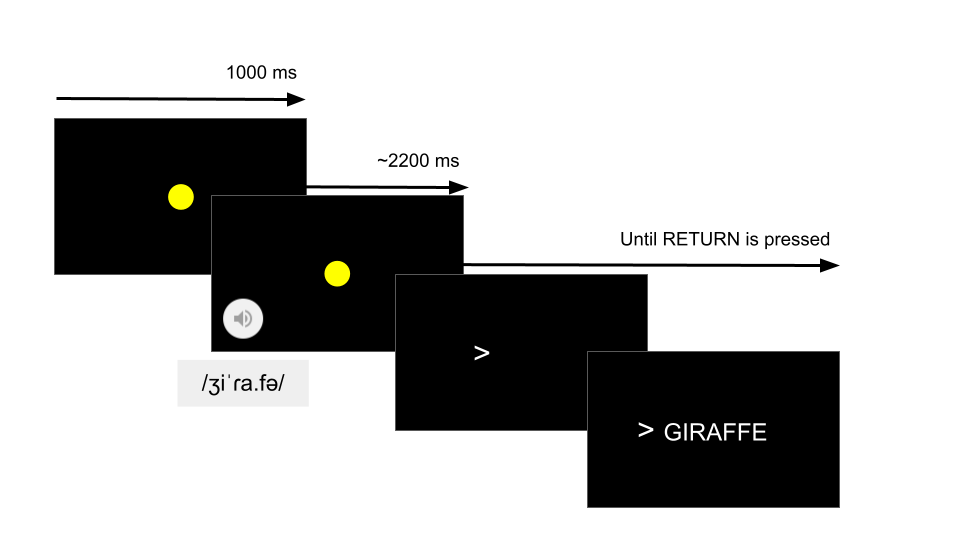
\includegraphics{_assets/img/design.png}

}

\caption{Schematic representation of a trial in the experimental task}

\end{figure}%

\subsubsection{Data analysis}\label{data-analysis}

\paragraph{Data processing}\label{data-processing}

After data collection, participants answers were manually coded into the
following categories: \emph{Correct}, \emph{Typo}, \emph{Wrong},
\emph{False friend}, \emph{Other}. Responses were coded as
\emph{Correct} if the provided string of characters was identical to the
orthographic form of the correct translation. Trials were coded as
\emph{Typo} if the participant provided a string of characters only one
edit distance (addition, deletion, or substitution) apart from the
orthographic form of the correct translation (e.g., ``pengiun'' instead
of ``penguin''), as long as the response did not correspond to a
distinct English word. Responses were coded as \emph{False friend} if
the participant provided a phonologically similar incorrect translation.
Responses were coded as \emph{Other} (see Data analysis section for more
details). Both \emph{Correct} and \emph{Typo} responses were considered
as correct, while \emph{Wrong} and \emph{False friend} responses were
considered as incorrect. \emph{Other} responses were excluded from data
analysis. Trials in which participants took longer than 10 seconds to
respond were also excluded. Participants contributed a total of 9152
valid trials (5,694 in Catalan, 3,458 in Spanish). The task took
approximately 15 minutes to be completed.

\paragraph{Modelling approach and statistical
inference}\label{modelling-approach-and-statistical-inference}

We modelled the probability of participants guessing the correct
translation of each presented word using a generalised multilevel
Bayesian regression model with a Bernoulli logit link distribution. We
included as fixed effects the intercept, the main effects of
\emph{Frequency}, \emph{Similarity}, and \emph{CLPN}, and the two-way
interaction between \emph{Similarity} and \emph{CLPN}. We also included
participant-level random intercepts and slopes for the the main effects
and the interaction. Eq. 1 shows a formal description of the model.

\[
\begin{aligned}
&\textbf{Likelihood}  \\
y_{i} \sim & \text{Bernoulli}(p_{i}) \\ \\
&\textbf{Parameters}  \\
\text{Logit}(p_{i}) = &  \beta_{0[p,w]} + \beta_{1[p]} \text{Frequency}_{i} + \beta_{2[p]} \text{PTHN}_i + \beta_{3[p]} \text{Similarity}_i + \beta_{4[p]} (\text{PTHN}_i \times \text{Similarity}_i) \\
\beta_{0-6[p,w]} \sim & \mathcal{N}(\mu_{\beta_{j}}, \sigma_{\beta_{j}}) \text{, for participant } p \text{ in 1, ..., } P \text{ and  word } w \text{ in 1, ..., } W \\
\beta_{1-6[p]} \sim &  \mathcal{N}(\mu_{\beta_{j}}, \sigma_{\beta_{j}}) \text{, for participant } p \text{ in 1, ..., } P \\ \\
&\textbf{Prior}  \\
\mu_{\beta_{p,w}}  \sim &  \mathcal{N}(0, 0.1) \\
\sigma_{\beta_{p}},  \sigma_{\beta_{w}} \sim & \text{HalfCauchy}(0, 0.1) \\
\rho_{p}, \rho_{w} \sim & \text{LKJCorr}(8) \\
\end{aligned}
\]

To test the practical relevance of each predictor we followed
(\citeproc{ref-kruschke2018bayesian}{Kruschke \& Liddell, 2018}). We
first specified a region of practical equivalence (\emph{ROPE}) around
zero ({[}-0.1, +0.1{]}, in the logit scale). This area indicates the
values of the regression coefficients that we considered as equivalent
to zero. We then computed the 95\% posterior credible intervals (CrI) of
the regression coefficients of interest. Finally, we calculated the
proportion of the 95\% CrI that fell inside the ROPE. This proportion
indicates the probability that the true value of the coefficient is
equivalent to zero. All analyses were performed in R environment
(\citeproc{ref-rcoreteam2013language}{R Core Team, 2013}). We used the
tidyverse family of R packages
(\citeproc{ref-wickham2019welcome}{Wickham et al., 2019}) to process
data and to generate figures. We used the \texttt{brms} R package
(\citeproc{ref-burkner2017brms}{Bürkner, 2017}) using the
\texttt{cmdstanr} back-end to the Stan probabilistic language
(\citeproc{ref-carpenter2017stan}{Carpenter et al., 2017}) to estimate
and compare the models (see Appendix 1 for mode details on the models).

\subsection{Results}\label{results}

We collected data for a total of 6,446 trials completed by 72 unique
participants. Of those trials, 2,988 were provided by 36 unique
participants who listened to Catalan words, and 3,458 trials were
provided by 36 unique participants who listened to Spanish words. We
excluded trials in which participants did not enter any text (\emph{n} =
72), in which a response in a language other than English was provided
(e.g., \texttt{agua}, \emph{n} = 51), in which participants did not
provide a whole word (e.g., \texttt{f}, \emph{n} = 5), and in which
participants added comments to the experimenter (e.g., \texttt{unsure},
\emph{n} = 13). In addition, we excluded data from participants that
self-rated their oral and/or written skills in Catalan and Spanish, or
any other second language as four or higher in a five-point scale
(\emph{n} = 2), were diagnosed with a language (\emph{n} = 1), or did
not contribute more than 80\% of valid trials (\emph{n} = 9).

After applying trial-level and participant-level inclusion criteria, the
resulting dataset included 5,204 trials provided by 54 unique
participants. Of those trials, 2,602 were provided by 27 unique
participants who listened to Catalan words, and 2,604 trials were
provided by 32 unique participants who listened to Spanish words.
Responses given by English participants to Catalan presented words were
5.35 characters long on average (\emph{Median} = 5, \emph{SD} = 1.79,
Range = 1-14), while their translations to Spanish responses were 5.57
characters long on average (\emph{Median} = 5, \emph{SD} = 1.97, Range =
2-21).

\begin{longtable}{l|rrrrrrrr}

\caption{\label{tbl-results}}

\tabularnewline

\toprule
\multicolumn{1}{l}{} & \multicolumn{4}{c}{Correct responses} & \multicolumn{4}{c}{Incorrect responses} \\ 
\cmidrule(lr){2-5} \cmidrule(lr){6-9}
\multicolumn{1}{l}{} & Correct & (\%) & Typo & (\%) & Wrong & (\%) & False friend & (\%) \\ 
\midrule\addlinespace[2.5pt]
\multicolumn{9}{l}{Experiment 1} \\ 
\midrule\addlinespace[2.5pt]
cat-ENG & $429$ & ($16.47$) & $11$ & ($0.42$) & $2,082$ & ($79.95$) & $82$ & ($3.15$) \\ 
spa-ENG & $374$ & ($14.37$) & $2$ & ($0.08$) & $2,117$ & ($81.36$) & $109$ & ($4.19$) \\ 
\midrule 
\emph{Sum} & $803$ & — & $13$ & — & $4,199$ & — & $191$ & — \\ 
\emph{Mean} & — & $15.42$ & — & $0.25$ & — & $80.66$ & — & $3.67$ \\ 
\midrule\addlinespace[2.5pt]
\multicolumn{9}{l}{Experiment 2} \\ 
\midrule\addlinespace[2.5pt]
cat-SPA & $780$ & ($46.93$) & $20$ & ($1.20$) & $736$ & ($44.28$) & $126$ & ($7.58$) \\ 
\midrule 
\emph{Sum} & $780$ & — & $20$ & — & $736$ & — & $126$ & — \\ 
\emph{Mean} & — & $46.93$ & — & $1.20$ & — & $44.28$ & — & $7.58$ \\ 
\midrule\addlinespace[2.5pt]
\multicolumn{9}{l}{Experiment 3} \\ 
\midrule\addlinespace[2.5pt]
cat-ENG & $477$ & ($18.01$) & $7$ & ($0.26$) & $1,986$ & ($75.00$) & $178$ & ($6.72$) \\ 
spa-ENG & $590$ & ($19.53$) & $6$ & ($0.20$) & $2,294$ & ($75.94$) & $131$ & ($4.34$) \\ 
\midrule 
\emph{Sum} & $1,067$ & — & $13$ & — & $4,280$ & — & $309$ & — \\ 
\emph{Mean} & — & $18.77$ & — & $0.23$ & — & $75.47$ & — & $5.53$ \\ 
\bottomrule

\end{longtable}

Table~\ref{tbl-dataset} shows a summary of participants' accuracy across
Experiments 1, 2, and 3. MCMC chains in the model showed strong evidence
of convergence (\(\hat{R}<1.01\)) (see Appendix 2 for more detailed
model diagnostics). Participants translating Catalan words and
participants translating Spanish words performed equivalently, as
indicated by the regression coefficient of \emph{Group} (\(\beta\) =
-0.199, 95\% CrI = {[}-0.512, 0.129{]}, \emph{p}(ROPE) = 0.238).
Overall, participants responded less accurately to words with more CLPNs
than to words with fewer CLPNs, regardless of the amount of phonological
similarity between the presented word and its translation. This is
indicated by the size of the regression coefficient of the two-way
interaction between \emph{Similarity} and \emph{CLPN} (\(\beta\) =
-0.653, 95\% CrI = {[}-0.973, -0.313{]}, \emph{p}(ROPE) = 0). As
anticipated, participants' performance benefited from an increase in
\emph{Similarity} (\(\beta\) = 7.133, 95\% CrI = {[}6.606, 7.735{]},
\emph{p}(ROPE) = 0), while the number of \emph{CLND} had the opposite
effect (\(\beta\) = 0.009, 95\% CrI = {[}-0.11, 0.111{]}, \emph{p}(ROPE)
= 0.925). Figure~\ref{fig-epreds-1} illustrates the posterior of the
average predictions of the model for words with different values of
\emph{Similarity} and \emph{CLPN}. Figure~\ref{fig-coefs} shows a
graphic summary of the posterior distribution of the regression
coefficients of interest.

\begin{longtable}{l|rrrrrrrrr}

\caption{\label{tbl-dataset}}

\tabularnewline

\toprule
\multicolumn{1}{l}{} &  & \multicolumn{4}{c}{Accuracy (\%)} & \multicolumn{4}{c}{Valid trials} \\ 
\cmidrule(lr){3-6} \cmidrule(lr){7-10}
\multicolumn{1}{l}{} & N & Mean & SD & SE & Range & Mean & N trials & SD & Range \\ 
\midrule\addlinespace[2.5pt]
\multicolumn{10}{l}{Experiment 1} \\ 
\midrule\addlinespace[2.5pt]
spa-ENG & $27$ & $15.86$ & $5.20$ & $3.05$ & $8.82$–$28.71$ & $96.37$ & $2,602$ & $2.88$ & $87$–$98$ \\ 
cat-ENG & $32$ & $18.48$ & $4.89$ & $3.27$ & $10.84$–$32.56$ & $81.38$ & $2,604$ & $3.17$ & $71$–$83$ \\ 
\midrule 
\emph{Sum} & $59$ & — & — & — & — & — & $5,206$ & — & $158$ \\ 
\emph{Mean} & — & $17.17$ & $5.05$ & $3.16$ & — & $8,887.27$ & — & $302.71$ & — \\ 
\midrule\addlinespace[2.5pt]
\multicolumn{10}{l}{Experiment 2} \\ 
\midrule\addlinespace[2.5pt]
cat-SPA & $21$ & $48.30$ & $5.29$ & $10.54$ & $38.27$–$58.97$ & $79.14$ & $1,662$ & $3.14$ & $72$–$82$ \\ 
\midrule 
\emph{Sum} & $21$ & — & — & — & — & — & $1,662$ & — & $72$ \\ 
\emph{Mean} & — & $48.30$ & $5.29$ & $10.54$ & — & $7,914.29$ & — & $313.51$ & — \\ 
\midrule\addlinespace[2.5pt]
\multicolumn{10}{l}{Experiment 3} \\ 
\midrule\addlinespace[2.5pt]
spa-ENG & $31$ & $20.92$ & $8.29$ & $3.76$ & $5.88$–$44.12$ & $97.45$ & $3,021$ & $1.80$ & $88$–$98$ \\ 
cat-ENG & $32$ & $19.74$ & $4.94$ & $3.49$ & $10.34$–$27.91$ & $82.75$ & $2,648$ & $0.44$ & $82$–$83$ \\ 
\midrule 
\emph{Sum} & $63$ & — & — & — & — & — & $5,669$ & — & $170$ \\ 
\emph{Mean} & — & $20.33$ & $6.62$ & $3.62$ & — & $9,010.08$ & — & $112.22$ & — \\ 
\bottomrule

\end{longtable}

\begin{figure}

\centering{

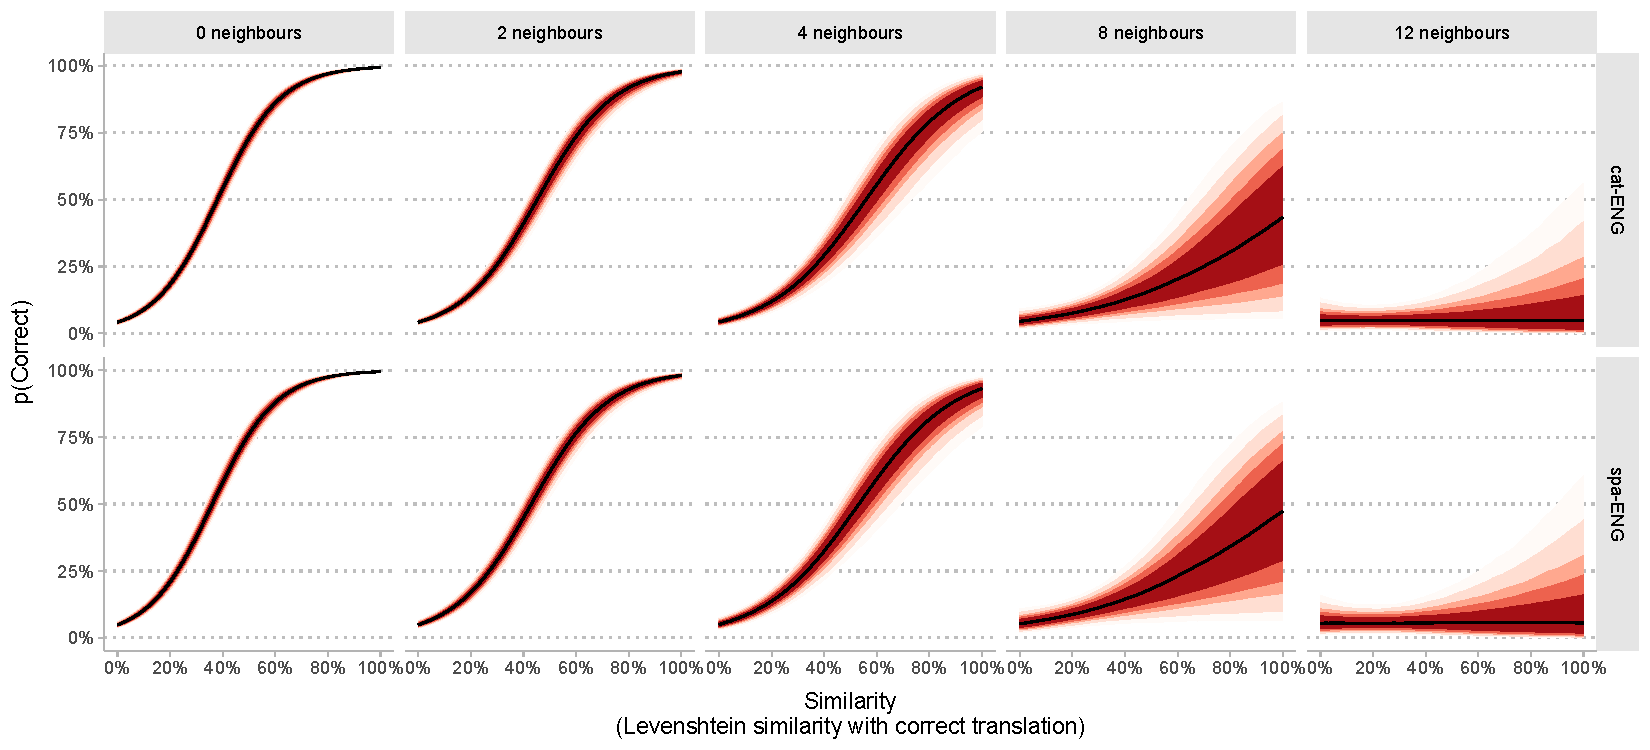
\includegraphics{manuscript_files/figure-pdf/fig-epreds-1-1.pdf}

}

\caption{\label{fig-epreds-1}Posterior model-predicted mean accuracy in
Experiment 1. Predictions were generated from 4,000 posterior samples,
extracted for different values of \emph{CLPN} (0, 2, 4, 8, 12) and
\emph{Similarity} (1-100). Predictions are plotted separately for
English participants translating Catalan words, and for English
participants translating Spanish words. Lines indicate mean predictions,
and intervals indicate 95\%, 89\%, 78\%, 67\%, and 50\% credible
intervals (CrI).}

\end{figure}%

\subsection{Discussion}\label{discussion}

In the present experiment, we investigated the extent to which the
phonological similarity between translation equivalents is sufficient
for successful word translation, in the absence of semantic knowledge.
We tested two groups of monolingual British English natives in a
translation task that involved words in Catalan or Spanish, two
languages participants reported having no prior familiarity with.
Participants benefited strongly from phonological similarity when the
correct translation of the presented words in Catalan or Spanish had few
English phonological neighbours with higher lexical frequency. This
suggests that, in the absence of distractors, even naïve participants
can efficiently use phonological similarity to succeed in a translation
task. Our results suggest that word-to-word connections at the
phonological level might play a strong role during L2 speech
comprehension, specially in low-proficiency listeners.

\section{Experiment 2}\label{experiment-2}

Results in Experiment 1 suggest that English natives were able to
exploit the phonological similarity between unfamiliar words in Catalan
and Spanish to provide accurate translations to English. English, a
Germanic language, is relatively distant from Catalan and Spanish, two
Romance languages. English shares fewer cognates with Catalan and
Spanish than it does with typologically closer languages, like Dutch and
German. In Experiment 2, we investigated whether listeners of an
unfamiliar but typologically closer language benefit more strongly from
phonological similarity when performing the same task as in Experiment
1. To this aim, we presented Spanish participants, who reported
little-to-no prior familiarity with Catalan, with Catalan words.

\subsection{Methods}\label{methods-1}

Participants in Spain were contacted via announcements in Faculties, and
were compensated 5€ or an Amazon voucher for the same value.
Participants gave informed consent before providing any data and the
study was conducted in accordance with ethical standards of the
Declaration of Helsinki and the protocol was approved by the Drug
Research Ethical Committee (CEIm) of the IMIM Parc de Salut Mar
(2020/9080/I). Data collection took place from June 08th, 2020 to June
28th, 2020. We collected data from 33 Spanish native participants living
in Spain (\emph{Mean} = 21.85 years, \emph{SD} = 3, Range = 18-33, 28, 5
female). Stimuli were the same list of Catalan stimuli as in Experiment
1. Procedure and data analysis were identical as in Experiment 1.

\subsection{Results}\label{results-1}

We collected data for a total of 5,412 trials completed by 33 unique
participants. We excluded trials in which participants did not enter any
text (\emph{n} = 44), in which a response in a language other than
English was provided (e.g., \texttt{agua}, \emph{n} = 51), in which
participants did not provide a whole word (e.g., \texttt{f}, \emph{n} =
7), and in which participants added comments to the experimenter (e.g.,
\texttt{unsure}, (\emph{n} = 1). In addition, we excluded data from
participants that self-rated their oral and/or written skills in Catalan
and Spanish, or any other second language as four or higher in a
five-point scale (\emph{n} = 22), were diagnosed with a language
(\emph{n} = 1), or did not contribute more than 80\% of valid trials
(\emph{n} = 9). After applying trial-level and participant-level
inclusion criteria, the resulting dataset included 1,662 trials provided
by 42 unique participants. Of those trials, 1,662 were provided by 21
unique participants who listened to Catalan words, and 1,662 trials were
provided by 21 unique participants who listened to Spanish words.
Responses given by participants were 5.6 characters long on average
(\emph{Median} = 5, \emph{SD} = 1.6, Range = 2-12).

MCMC chains in the model showed strong evidence of convergence
(\(\hat{R}<1.01\)) (see Appendix 2 for more detailed model diagnostics).
Overall, participants responded less accurately to words with more CLPNs
than to words with fewer CLPNs, regardless of the amount of phonological
similarity between the presented word and its translation. This is
indicated by the size of the regression coefficient of the two-way
interaction between \emph{Similarity} and \emph{CLPN} (\(\beta\) =
-0.409, 95\% CrI = {[}-0.895, 0.111{]}, \emph{p}(ROPE) = 0.081). As
anticipated, participants' performance benefited from an increase in
\emph{Similarity} (\(\beta\) = 9.274, 95\% CrI = {[}8.473, 10.269{]},
\emph{p}(ROPE) = 0), while the number of \emph{CLND} had the opposite
effect (\(\beta\) = -0.069, 95\% CrI = {[}-0.353, 0.192{]},
\emph{p}(ROPE) = 0.492). Figure~\ref{fig-epreds-1} illustrates the
posterior of the average predictions of the model for words with
different values of \emph{Similarity} and \emph{CLPN}.

\begin{figure}

\centering{

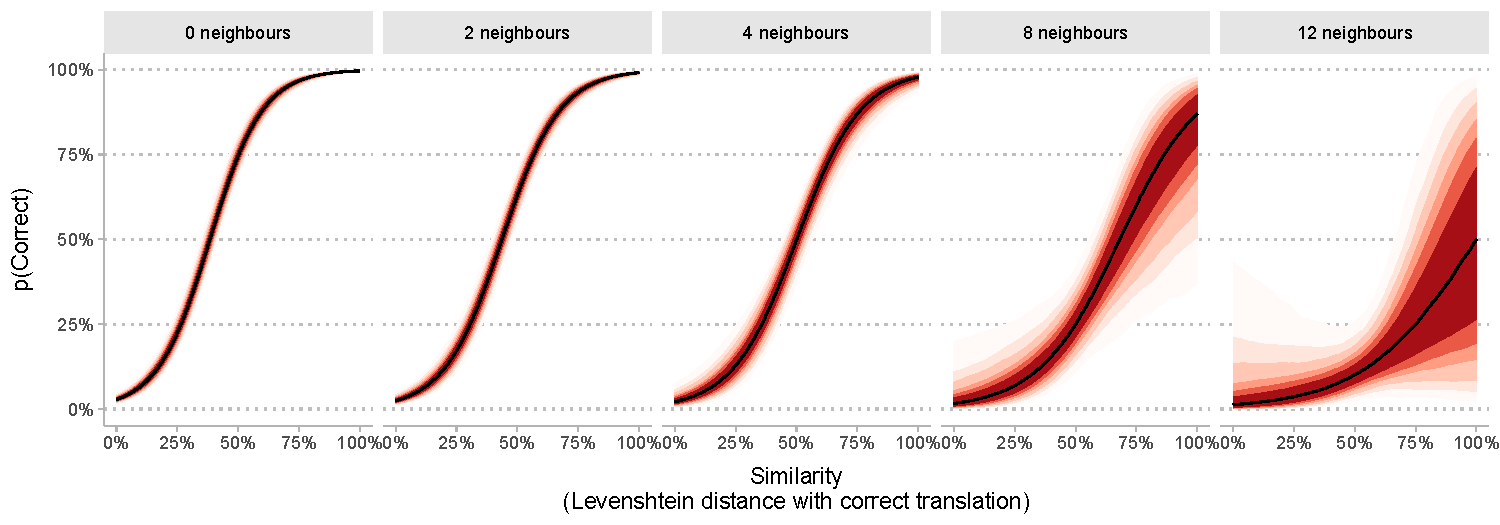
\includegraphics{manuscript_files/figure-pdf/fig-epreds-2-1.pdf}

}

\caption{\label{fig-epreds-2}Posterior model-predicted mean accuracy in
Experiment 1. Predictions were generated from 4,000 posterior samples,
extracted for different values of \emph{CLPN} (0, 2, 4, 8, 12) and
\emph{Similarity} (1-100). Predictions are plotted separately for
English participants translating Catalan words, and for English
participants translating Spanish words. Lines indicate mean predictions,
and intervals indicate 95\%, 89\%, 78\%, 67\%, and 50\% credible
intervals (CrI).}

\end{figure}%

\subsection{Discussion}\label{discussion-1}

Experiment 2 was an extension of Experiment 1 to a population of
monolinguals whose native language is typologically similar to the
presented language. Particularly, we presented Catalan words to Spanish
native speakers who were reportedly unfamiliar with Catalan. Our results
indicate a similar pattern of results as those in Experiment 1:
participants were able to provide correct translations of presented
Catalan words, provided that the Catalan words shared some degree of
phonological similarity with their Spanish translation, and that the
number of phonological neighbours with higher lexical frequency was
reduced. In contrasts with the results in Experiment 1, the positive
impact of phonological similarity on participants' performance in
Experiment 2 was more resilient to the interference of phonological
neighbours. English natives in Experiment 1 provided significantly less
accuracy responses when more than four phonological neighbors were
present (even when translating high-similarity words), compared to when
only one or neighbour were present. Spanish participants in Experiment 2
benefited from phonological similarity, even when eight neighbours were
present. Spanish participants' performance declined after 8 neighbours,
and was evident at 12 neighbours. Overall, this suggests that
participants in Experiment 2, who were natives of a typologically
similar language (Spanish) to the presented language (Catalan) benefited
more strongly from phonological similarity than participants in
Experiment 1, who were natives of typologically less similar language
(English) to the presented language (Catalan, Spanish).

Participants from both Experiment 1 and 2 benefited strongly from
phonological similarity to correctly translate words from a non-native,
reportedly unfamiliar language. This pattern of results holds for most
of the presented stimuli, but some low-similarity Catalan and Spanish
words were responded to surprisingly accurately by English listeners.
Given that participants were reportedly unfamiliar with both languages,
it was expected that participants would be very unlikely to provide
correct translations for words sharing little to no phonological
similarity to their correct translation. Table~\ref{tbl-surprises} a
list of Catalan and Spanish words to which participants provided
responses with \(\geq\) 10 average accuracy.

\begin{longtable}{l|rr}

\caption{\label{tbl-surprises}List of items with unexpectedly high
accuracy: the Levenshtein similarityscore betwen th presented word (in
Catalan or Spanish) and their correct Enlgish or Spanish translation is
zero, but participants, who are reportedly unfamiliar with the presented
language, were on average \textgreater10\% likely to guess the correct
translation.}

\tabularnewline

\toprule
\multicolumn{1}{l}{} & Accuracy (\%) & SE \\ 
\midrule\addlinespace[2.5pt]
\multicolumn{3}{l}{Experiment 1 - cat-ENG} \\ 
\midrule\addlinespace[2.5pt]
cavall /kəβaʎ/ - horse /hɔs/ & $17.14$ & $6.37$ \\ 
llibre /ʎiβɾə/ - book /bʊk/ & $17.14$ & $6.37$ \\ 
camisa /kəmizə/ - shirt /ʃɜt/ & $16.67$ & $6.21$ \\ 
poma /poma/ - apple /æpl/ & $16.67$ & $6.21$ \\ 
cama /kamə/ - leg /lɛg/ & $11.11$ & $5.24$ \\ 
\midrule\addlinespace[2.5pt]
\multicolumn{3}{l}{Experiment 1 - spa-ENG} \\ 
\midrule\addlinespace[2.5pt]
pantalón /paŋtalon/ - trousers /traʊzəz/ & $77.42$ & $7.51$ \\ 
naranja /naɾaŋxa/ - orange /ɒrɪnʤ/ & $41.94$ & $8.86$ \\ 
leche /leʧe/ - milk /mɪlk/ & $35.48$ & $8.59$ \\ 
toro /toɾo/ - bull /bʊl/ & $33.33$ & $8.61$ \\ 
libro /liβɾo/ - book /bʊk/ & $30.00$ & $8.37$ \\ 
cebra /θebɾa/ - zebra /zibrə/ & $29.03$ & $8.15$ \\ 
pan /pan/ - bread /brɛd/ & $29.03$ & $8.15$ \\ 
pollo /poʎo/ - chicken /ʧɪkɪn/ & $26.67$ & $8.07$ \\ 
jirafa /xiɾafa/ - giraffe /ʤɪrɑf/ & $20.69$ & $7.52$ \\ 
perro /pero/ - dog /dɒɡ/ & $16.13$ & $6.61$ \\ 
pluma /pluma/ - feather /fɛðə/ & $16.13$ & $6.61$ \\ 
puerta /pwerta/ - door /dɔ/ & $16.13$ & $6.61$ \\ 
pie /pje/ - foot /fʊt/ & $12.90$ & $6.02$ \\ 
caballo /kaβaʎo/ - horse /hɔs/ & $10.34$ & $5.66$ \\ 
bocadillo /bokadiʎo/ - sandwich /sænwɪʤ/ & $10.00$ & $5.48$ \\ 
globo /ɡloβo/ - balloon /bəlun/ & $10.00$ & $5.48$ \\ 
\midrule\addlinespace[2.5pt]
\multicolumn{3}{l}{Experiment 2 - cat-SPA} \\ 
\midrule\addlinespace[2.5pt]
fulla /fuʎə/ - hoja /oxa/ & $30.43$ & $9.59$ \\ 
ull /uʎ/ - ojo /oxo/ & $21.74$ & $8.60$ \\ 
got /gɔt/ - vaso /baso/ & $20.00$ & $8.00$ \\ 
entrepà /entɾəpa/ - bocadillo /bokadiʎo/ & $13.04$ & $7.02$ \\ 
mirall /miɾaʎ/ - espejo /espexo/ & $12.50$ & $6.75$ \\ 
\bottomrule

\end{longtable}

It is likely that participants had prior knowledge of these words
despite having reported little to no familiarity with the presented
language (Catalan or Spanish). One possibility is that participants had
previously encountered these words embedded in English linguistic input.
Spanish words percolate English speech with relative frequency, via
different sources such as popular culture, songs, TV programs, etc. In
addition, words from languages other than Spanish, but with high
similarity to the Spanish words (e.g., cognates from Italian or French)
might appear in English speech as well. Such prior knowledge might not
be specific to the low-similarity words highlighted before. Participants
may also have had prior knowledge about higher-similarity words, which
could have contributed to participants responding to such words more
accurately than without such prior knowledge. In the case of
higher-similarity words, it is more difficult to disentangle the extent
to which participants' accuracy is a function of pure phonological
similarity, or prior knowledge they had about the meaning of Spanish
words. To investigate this issue, we run Experiment 3.

{[}ADD HERE LEXICAL FREQUENCY OF CATALAN AND SPANISH WORDS IN ENGLISH,
AND OF CATALAN WORDS IN SPANISH{]}

\section{Experiment 3}\label{experiment-3}

Experiment 3 is a replication of Experiment 1, in which we collected
additional data about participants' prior familiarity with the presented
Catalan and Spanish words, in addition to the same translation task
presented to participants in Experiment 1.

\subsection{Methods}\label{methods-2}

Data collection took place from October 22th, 2022 to October 23th,
2022. We collected data from 64 British English native participants
living in United Kingdom (\emph{Mean} = 22.02 years, \emph{SD} = 2.49,
Range = 18-26, 36, 28 female).

Participants were recruited via Prolific (5£ compensation) and SONA
(compensation in academic credits), and gave informed consent before
providing any data and the study was conducted in accordance with
ethical standards of the Declaration of Helsinki and the protocol was by
the University of Oxford Medical Sciences Inter-Divisional Research
Ethics Committee (IDREC) (R60939/RE007). Participants were asked to
complete the experiment using a laptop in a quiet place with good
internet connection. Stimuli were the same list of Catalan stimuli as in
Experiment 1.

The experiment was implemented online using Qualtrics (Qualtrics, Provo,
UT). This platform was chosen to allow easier presentation of survey
questions aimed to probe prior understanding of the presented words and
participants' confidence ratings of their answers. With the exception of
these additional questions, we attempted to replicate the procedure of
Experiment 1 as closely as possible. The Spanish and Catalan audio
stimuli used were identical the materials in Experiment 1. Participants
were randomly assigned to the Catalan or Spanish lists. The Catalan list
had 83 trials and the Spanish list had 99 trials. Participants first
completed the consent form followed by the questionnaire about
demographic status, language background and set up. They then proceeded
to the experimental task.

On each trial, participants listened to the audio stimulus by clicking
on the \texttt{PLAY} button. For comparability to the PsychoPy version,
participants were only allowed to play the audio one time. Participants
were explicitly told that they would be only allowed to listen once. The
\texttt{PLAY} button vanished after one playthrough. Participants then
had to answer three questions based on the audio they had heard on that
trial. These questions were presented on the same page, directly below
the audio player. They were first asked whether or not they knew the
presented word (multiple choice---\emph{yes}/\emph{no}). Regardless of
their answer on the first question, participants were asked what they
thought the translation of the word was in English (or their best
guess), and instructed to type their answer in the provided text box.
Finally, they were asked to rate how confident they were in their answer
on a scale of 0 to 7, where 7 was ``very confident'' and 0 was ``not
confident''. There was no time limit on the response phase. All
questions had to be answered to proceed to the next trial.

Participants first completed 5 practice trials with English words as the
audio stimulus (ambulance, cucumber, elephant, pear, turtle). The words
were recorded by a female native speaker of English. These trials acted
as attention checks, as participants should always answer ``yes'' to the
first question on prior word knowledge and be able to accurately
transcribe the word they heard. Following the practice phase,
participants completed the test phase where they heard either Spanish
words or Catalan words.

\subsection{Results}\label{results-2}

We collected data for a total of 6,016 trials completed by 64 unique
participants. Of those trials, 2,752 were provided by 32 unique
participants who listened to Catalan words, and 3,264 trials were
provided by 32 unique participants who listened to Spanish words. We
excluded trials in which participants did not enter any text (\emph{n} =
), in which a response in a language other than English was provided
(e.g., \texttt{agua}, \emph{n} = ), in which participants did not
provide a whole word (e.g., \texttt{f}, \emph{n} = ), and in which
participants added comments to the experimenter (e.g., \texttt{unsure},
(\emph{n} = ). In addition, we excluded data from participants that
self-rated their oral and/or written skills in Catalan and Spanish, or
any other second language as four or higher in a five-point scale
(\emph{n} = 2), were diagnosed with a language (\emph{n} = 0), or did
not contribute more than 80\% of valid trials (\emph{n} = 1).

After applying trial-level and participant-level inclusion criteria, the
resulting dataset included 6,290 trials provided by 62 unique
participants. Of those trials, 3,145 were provided by 31 unique
participants who listened to Catalan words, and 2,743 trials were
provided by 32 unique participants who listened to Spanish words.

INSERT PRIOR KNOWLEDGE FILTER

Responses given by English participants to Catalan presented words were
5.52 characters long on average (\emph{Median} = 5, \emph{SD} = 1.75,
Range = 1-17), while their translations to Spanish responses were 5.41
characters long on average (\emph{Median} = 5, \emph{SD} = 1.77, Range =
1-20).

MCMC chains in the model showed strong evidence of convergence
(\(\hat{R}<1.01\)) (see Appendix 2 for more detailed model diagnostics).
Overall, participants reported prior knowledge more often for that
Spanish words with unexpectedly high accuracy (see Discussion in
Experiment 2) than for words with expected accuracy (see
Figure~\ref{fig-knowledge}). Participants reported prior knowledge of
Catalan words with unexpected accuracy as often as those with expected
accuracy. This suggests that participants in Experiment 1 may have
relied, to some extent, on their prior knowledge about form-meaning
mappings to correctly translate some Spanish words. To isolate such an
effect of prior Spanish knowledge, we run the same analysis as in
Experiment 1 on the newly collected translations from Experiment 3, now
excluding responses to words in which participants reported prior
knowledge.

\begin{figure}

\centering{

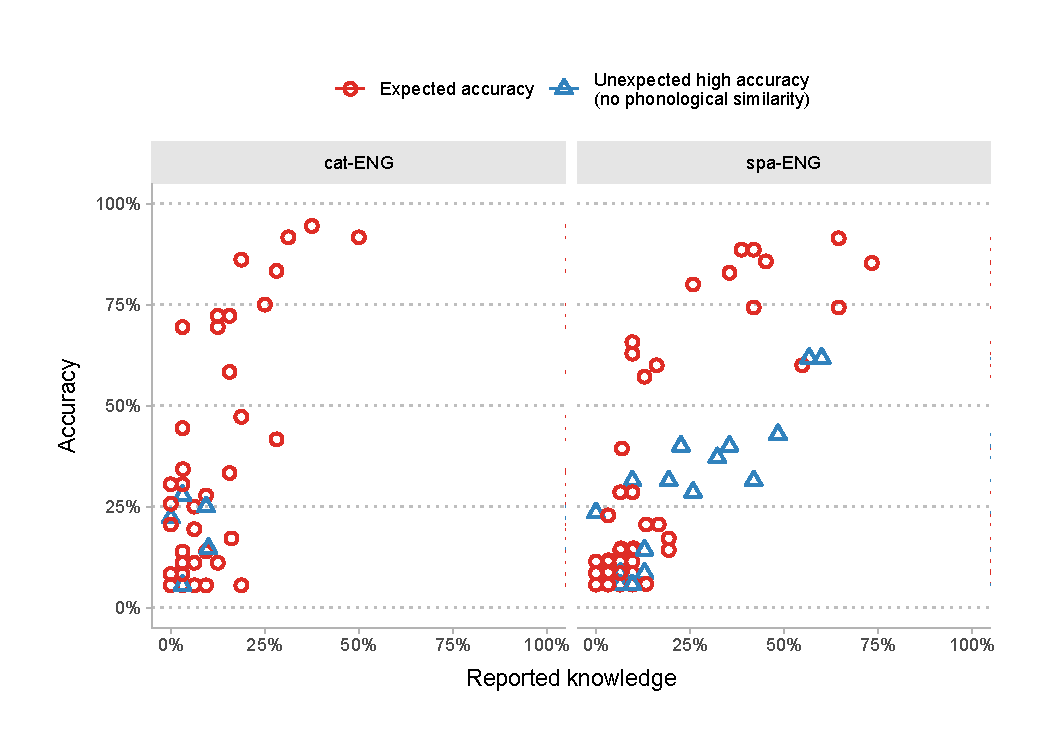
\includegraphics{manuscript_files/figure-pdf/fig-knowledge-1.pdf}

}

\caption{\label{fig-knowledge}Catalan/Spanish prior word knowledge as
reported by English native participants in Experiment 3. (A) Average
proportion of participants that reported prior knowledge for words with
surprisingly high accuracy (no phonological similarity with the correct
translation, accuracy higher than 10\%), and for words with expected
accuracy (low similarity-low accuracy, or high similarity-high
accuracy). (B) Average accuracy for words with expected and unexpected
accuracy.}

\end{figure}%

Participants translating Catalan words and participants translating
Spanish words, as indicated by the regression coefficient of
\emph{Group} (\(\beta\) = -0.049, 95\% CrI = {[}-0.388, -0.32{]},
\emph{p}(ROPE) = 0.426). Overall, participants responded less accurately
to words with more CLPNs than to words with fewer CLPNs, regardless of
the amount of phonological similarity between the presented word and its
translation. This is indicated by the size of the regression coefficient
of the two-way interaction between \emph{Similarity} and \emph{CLPN}
(\(\beta\) = -0.665, 95\% CrI = {[}-1.068, -0.32{]}, \emph{p}(ROPE) =
0.002). As anticipated, participants' performance benefited from an
increase in \emph{Similarity} (\(\beta\) = 7.585, 95\% CrI = {[}7.043,
8.24{]}, \emph{p}(ROPE) = 0), while the number of \emph{CLND} had the
opposite effect (\(\beta\) = -0.049, 95\% CrI = {[}-0.203, 0.086{]},
\emph{p}(ROPE) = 0.753). Figure~\ref{fig-epreds-1} illustrates the
posterior of the average predictions of the model for words with
different values of \emph{Similarity} and \emph{CLPN}.

\begin{figure}

\centering{

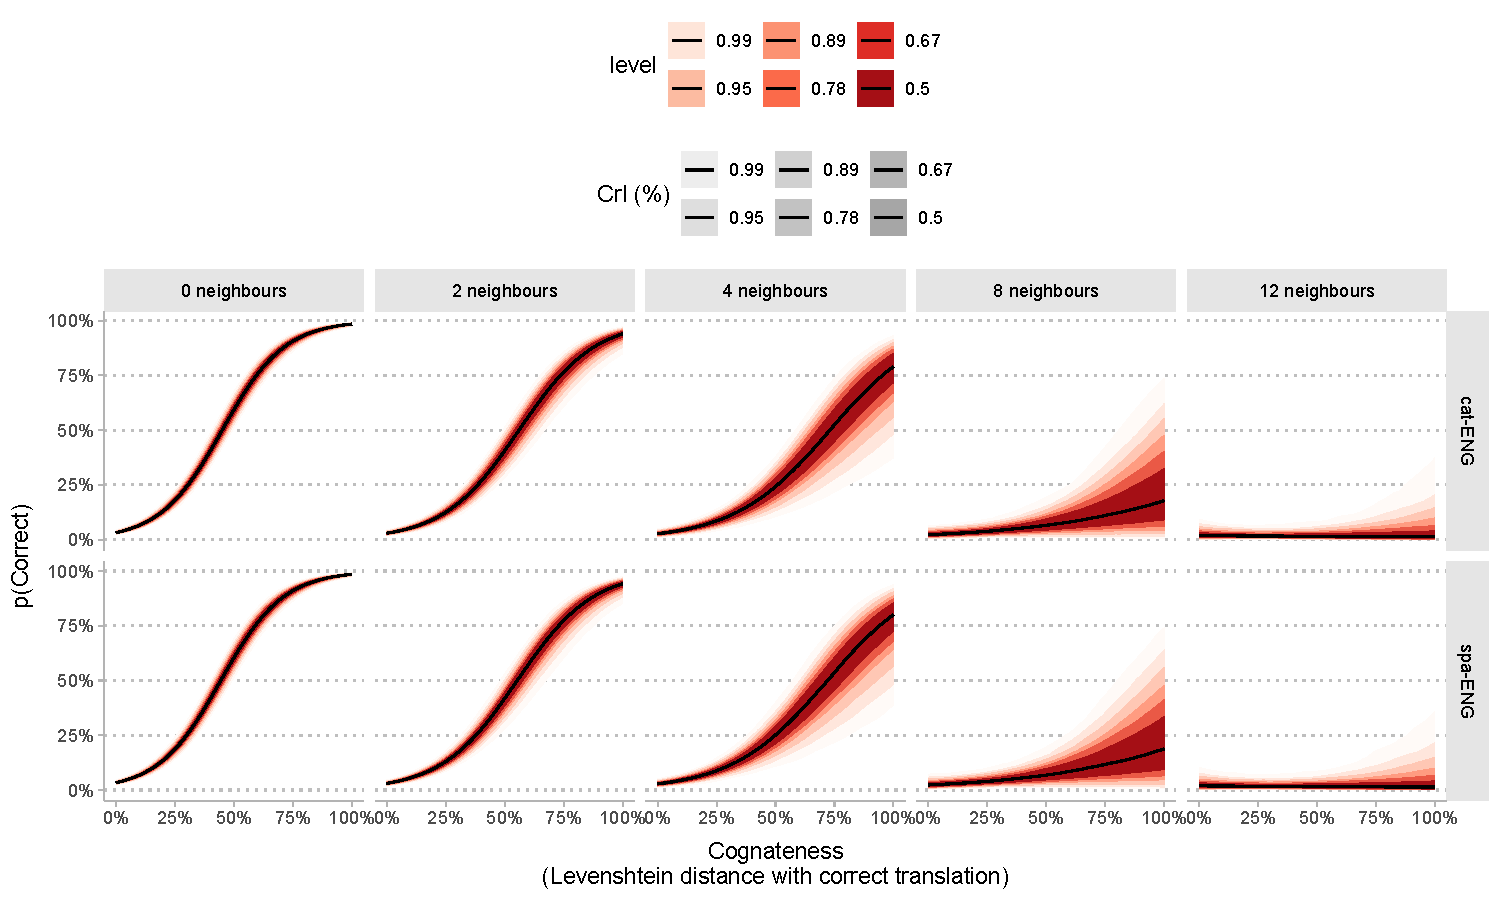
\includegraphics{manuscript_files/figure-pdf/fig-epreds-3-1.pdf}

}

\caption{\label{fig-epreds-3}Posterior model-predicted mean accuracy in
Experiment 2. Predictions were generated from 4,000 posterior samples,
extracted for different values of \emph{CLPN} (0, 2, 4, 8, 12) and
\emph{Similarity} (1-100). Predictions are plotted separately for
English participants translating Catalan words, and for English
participants translating Spanish words. Lines indicate mean predictions,
and intervals indicate 95\%, 89\%, 78\%, 67\%, and 50\% credible
intervals (CrI).}

\end{figure}%

\subsection{Discussion}\label{discussion-2}

\section{Joint analyses}\label{joint-analyses}

Across Experiments 1 and 3, we found strong evidence that participants
efficiently exploited phonological similarity to provide accurate
translations for words in an unfamiliar language, provided that few
phonological neighbours of higher lexical frequency were present.
Figure~\ref{fig-coefs} summarizes the posterior distribution of the
regression coefficients of the models in Experiments 1 to 3.

\begin{figure}

\centering{

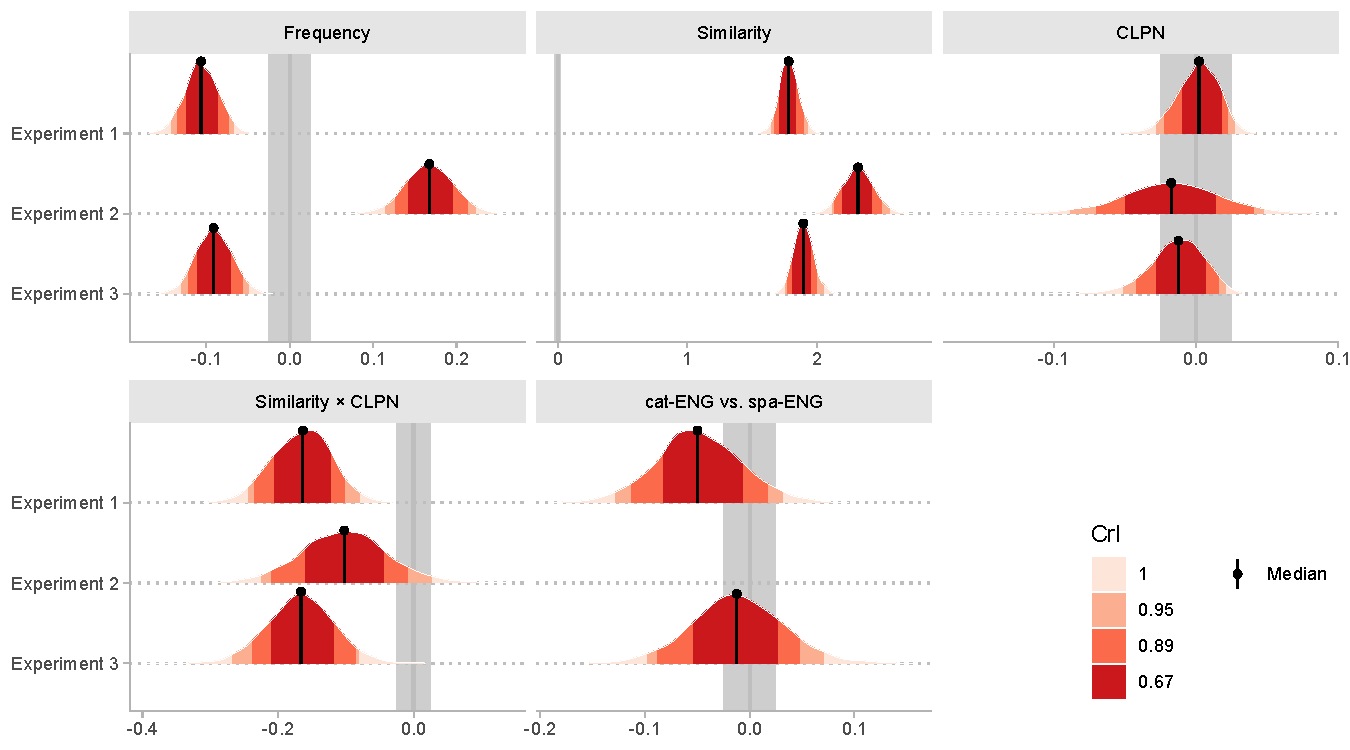
\includegraphics{manuscript_files/figure-pdf/fig-coefs-1.pdf}

}

\caption{\label{fig-coefs}}

\end{figure}%

\section{General discussion}\label{general-discussion}

This type of cross-linguistic similarity has also been extremely
informative for the study of bilingual lexical processing: words that
share high form-similarity with their translations are processed faster
and more accurately than words sharing lower phonological similarity.
This phenomenon has provided strong evidence in favour of the
language-non selective hypothesis of bilingual lexical access, which
states that bilinguals activate lexical representations in both
languages, even during monolingual situations. This facilitation effect
has been reported for comprehension
(\citeproc{ref-dijkstra2010cross}{Dijkstra et al., 2010};
\citeproc{ref-midgley2011effects}{Midgley et al., 2011};
\citeproc{ref-thierry2007brain}{Thierry \& Wu, 2007}), production
(\citeproc{ref-costa2000cognate}{Costa et al., 2000}), learning
(\citeproc{ref-de2000hard}{De Groot \& Keijzer, 2000};
\citeproc{ref-elias2022crosslanguage}{Elias \& Degani, 2022};
\citeproc{ref-lotto1998effects}{Lotto \& De Groot, 1998};
\citeproc{ref-valente2018does}{Valente et al., 2018}), and translation
(\citeproc{ref-christoffels2006memory}{Christoffels et al., 2006}).

\section{References}\label{references}

\phantomsection\label{refs}
\begin{CSLReferences}{1}{0}
\bibitem[\citeproctext]{ref-best2001discrimination}
Best, C. T., McRoberts, G. W., \& Goodell, E. (2001). Discrimination of
non-native consonant contrasts varying in perceptual assimilation to the
listener's native phonological system. \emph{The Journal of the
Acoustical Society of America}, \emph{109}(2), 775--794.

\bibitem[\citeproctext]{ref-best1988examination}
Best, C. T., McRoberts, G. W., \& Sithole, N. M. (1988). Examination of
perceptual reorganization for nonnative speech contrasts: Zulu click
discrimination by english-speaking adults and infants. \emph{Journal of
Experimental Psychology: Human Perception and Performance},
\emph{14}(3), 345.

\bibitem[\citeproctext]{ref-broersma2021praat}
Broersma, P., \& Weenink, D. (2021). \emph{Praat: Doing phonetics by
computer {[}{Computer} program{]}} (Version 6.1.54).
\url{http://www.praat.org/}

\bibitem[\citeproctext]{ref-burkner2017brms}
Bürkner, P.-C. (2017). Brms: {An R} package for {Bayesian} multilevel
models using {Stan}. \emph{Journal of Statistical Software},
\emph{80}(1), 1--28.

\bibitem[\citeproctext]{ref-carpenter2017stan}
Carpenter, B., Gelman, A., Hoffman, M. D., Lee, D., Goodrich, B.,
Betancourt, M., Brubaker, M., Guo, J., Li, P., \& Riddell, A. (2017).
Stan: {A} probabilistic programming language. \emph{Journal of
Statistical Software}, \emph{76}(1), 1--32.

\bibitem[\citeproctext]{ref-christoffels2006memory}
Christoffels, I. K., De Groot, A. M., \& Kroll, J. F. (2006). Memory and
language skills in simultaneous interpreters: {The} role of expertise
and language proficiency. \emph{Journal of Memory and Language},
\emph{54}(3), 324--345.

\bibitem[\citeproctext]{ref-costa2000cognate}
Costa, A., Caramazza, A., \& Sebastian-Galles, N. (2000). The cognate
facilitation effect: Implications for models of lexical access.
\emph{Journal of Experimental Psychology: Learning, Memory, and
Cognition}, \emph{26}(5), 1283.

\bibitem[\citeproctext]{ref-cutler2004patterns}
Cutler, A., Weber, A., Smits, R., \& Cooper, N. (2004). Patterns of
{English} phoneme confusions by native and non-native listeners.
\emph{The Journal of the Acoustical Society of America}, \emph{116}(6),
3668--3678.

\bibitem[\citeproctext]{ref-de2000hard}
De Groot, A. M., \& Keijzer, R. (2000). What is hard to learn is easy to
forget: The roles of word concreteness, cognate status, and word
frequency in foreign-language vocabulary learning and forgetting.
\emph{Language Learning}, \emph{50}(1), 1--56.

\bibitem[\citeproctext]{ref-dijkstra2010cross}
Dijkstra, T., Miwa, K., Brummelhuis, B., Sappelli, M., \& Baayen, H.
(2010). How cross-language similarity and task demands affect cognate
recognition. \emph{Journal of Memory and Language}, \emph{62}(3),
284--301.

\bibitem[\citeproctext]{ref-dufour2003lexical}
Dufour, S., \& Peereman, R. (2003). Lexical competition in phonological
priming: {Assessing} the role of phonological match and mismatch lengths
between primes and targets. \emph{Memory \& Cognition}, \emph{31},
1271--1283.

\bibitem[\citeproctext]{ref-dupoux1999epenthetic}
Dupoux, E., Kakehi, K., Hirose, Y., Pallier, C., \& Mehler, J. (1999).
Epenthetic vowels in japanese: A perceptual illusion? \emph{Journal of
Experimental Psychology: Human Perception and Performance},
\emph{25}(6), 1568.

\bibitem[\citeproctext]{ref-elias2022crosslanguage}
Elias, M., \& Degani, T. (2022). Cross-language interactions during
novel word learning: {The} contribution of form similarity and
participant characteristics. \emph{Bilingualism: Language and
Cognition}, 1--18.

\bibitem[\citeproctext]{ref-goldinger1989priming}
Goldinger, S. D., Luce, P. A., \& Pisoni, D. B. (1989). Priming lexical
neighbors of spoken words: {Effects} of competition and inhibition.
\emph{Journal of Memory and Language}, \emph{28}(5), 501--518.
\url{https://doi.org/10.1016/0749-596X(89)90009-0}

\bibitem[\citeproctext]{ref-hamburger1996phonological}
Hamburger, M., \& Slowiaczek, L. M. (1996). Phonological priming
reflects lexical competition. \emph{Psychonomic Bulletin \& Review},
\emph{3}(4), 520--525.

\bibitem[\citeproctext]{ref-kentner2015rhythmic}
Kentner, G. (2015). Rhythmic segmentation in auditory illusions-evidence
from cross-linguistic mondegreens. \emph{ICPhS}.

\bibitem[\citeproctext]{ref-kruschke2018bayesian}
Kruschke, J. K., \& Liddell, T. M. (2018). The {Bayesian New
Statistics}: {Hypothesis} testing, estimation, meta-analysis, and power
analysis from a {Bayesian} perspective. \emph{Psychonomic Bulletin \&
Review}, \emph{25}, 178--206.

\bibitem[\citeproctext]{ref-levenshtein1966binary}
Levenshtein, V. I. (1966). Binary codes capable of correcting deletions,
insertions, and reversals. \emph{Soviet Physics Doklady}, \emph{10},
707--710.

\bibitem[\citeproctext]{ref-lotto1998effects}
Lotto, L., \& De Groot, A. M. (1998). Effects of learning method and
word type on acquiring vocabulary in an unfamiliar language.
\emph{Language Learning}, \emph{48}(1), 31--69.

\bibitem[\citeproctext]{ref-luce1998recognizing}
Luce, P. A., \& Pisoni, D. B. (1998). Recognizing spoken words: {The}
neighborhood activation model. \emph{Ear and Hearing}, \emph{19}(1), 1.

\bibitem[\citeproctext]{ref-luce1990similarity}
Luce, P. A., Pisoni, D. B., \& Goldinger, S. D. (1990). \emph{Similarity
neighborhoods of spoken words.}

\bibitem[\citeproctext]{ref-marian2012clearpond}
Marian, V., Bartolotti, J., Chabal, S., \& Shook, A. (2012).
\emph{{CLEARPOND}: {Cross-linguistic} easy-access resource for
phonological and orthographic neighborhood densities}.

\bibitem[\citeproctext]{ref-midgley2011effects}
Midgley, K. J., Holcomb, P. J., \& Grainger, J. (2011). Effects of
cognate status on word comprehension in second language learners: {An
ERP} investigation. \emph{Journal of Cognitive Neuroscience},
\emph{23}(7), 1634--1647.

\bibitem[\citeproctext]{ref-otake2007interlingual}
Otake, T. (2007). Interlingual near homophonic words and phrases in L2
listening: Evidence from misheard song lyrics. \emph{Proceedings of the
16th International Congress of Phonetic Sciences (ICPhS 2007)},
777--780.

\bibitem[\citeproctext]{ref-otwinowska2019more}
Otwinowska, A., \& Szewczyk, J. M. (2019). The more similar the better?
Factors in learning cognates, false cognates and non-cognate words.
\emph{International Journal of Bilingual Education and Bilingualism}.

\bibitem[\citeproctext]{ref-peirce2019psychopy2}
Peirce, J., Gray, J. R., Simpson, S., MacAskill, M., Höchenberger, R.,
Sogo, H., Kastman, E., \& Lindeløv, J. K. (2019). {PsychoPy2}:
{Experiments} in behavior made easy. \emph{Behavior Research Methods},
\emph{51}(1), 195--203. \url{https://doi.org/10.3758/s13428-018-01193-y}

\bibitem[\citeproctext]{ref-peperkamp2008perceptual}
Peperkamp, S., Vendelin, I., \& Nakamura, K. (2008). On the perceptual
origin of loanword adaptations: Experimental evidence from japanese.
\emph{Phonology}, \emph{25}(1), 129--164.

\bibitem[\citeproctext]{ref-rcoreteam2013language}
R Core Team. (2013). \emph{R: {A Language} and {Environment} for
{Statistical Computing}}. R Foundation for Statistical Computing.
\url{http://www.R-project.org/}

\bibitem[\citeproctext]{ref-schepens2012distributions}
Schepens, J., Dijkstra, T., \& Grootjen, F. (2012). Distributions of
cognates in {Europe} as based on {Levenshtein} distance.
\emph{Bilingualism: Language and Cognition}, \emph{15}(1), 157--166.

\bibitem[\citeproctext]{ref-thierry2007brain}
Thierry, G., \& Wu, Y. J. (2007). Brain potentials reveal unconscious
translation during foreign-language comprehension. \emph{Proceedings of
the National Academy of Sciences}, \emph{104}(30), 12530--12535.

\bibitem[\citeproctext]{ref-valente2018does}
Valente, D., Ferré, P., Soares, A., Rato, A., \& Comesaña, M. (2018).
Does phonological overlap of cognate words modulate cognate acquisition
and processing in developing and skilled readers? \emph{Language
Acquisition}, \emph{25}(4), 438--453.

\bibitem[\citeproctext]{ref-van2014stringdist}
van der Loo, M. P. J. (2014). The stringdist package for approximate
string matching. \emph{The R Journal}, \emph{6}(1), 111--122.
\url{https://CRAN.R-project.org/package=stringdist}

\bibitem[\citeproctext]{ref-van2014subtlex}
Van Heuven, W. J., Mandera, P., Keuleers, E., \& Brysbaert, M. (2014).
{SUBTLEX-UK}: {A} new and improved word frequency database for {British
English}. \emph{Quarterly Journal of Experimental Psychology},
\emph{67}(6), 1176--1190.

\bibitem[\citeproctext]{ref-weber2004lexical}
Weber, A., \& Cutler, A. (2004). Lexical competition in non-native
spoken-word recognition. \emph{Journal of Memory and Language},
\emph{50}(1), 1--25.

\bibitem[\citeproctext]{ref-wickham2019welcome}
Wickham, H., Averick, M., Bryan, J., Chang, W., McGowan, L. D.,
François, R., Grolemund, G., Hayes, A., Henry, L., Hester, J., Kuhn, M.,
Pedersen, T. L., Miller, E., Bache, S. M., Müller, K., Ooms, J.,
Robinson, D., Seidel, D. P., Spinu, V., \ldots{} Yutani, H. (2019).
Welcome to the tidyverse. \emph{Journal of Open Source Software},
\emph{4}(43), 1686. \url{https://doi.org/10.21105/joss.01686}

\bibitem[\citeproctext]{ref-best2001discrimination}
Best, C. T., McRoberts, G. W., \& Goodell, E. (2001). Discrimination of
non-native consonant contrasts varying in perceptual assimilation to the
listener's native phonological system. \emph{The Journal of the
Acoustical Society of America}, \emph{109}(2), 775--794.

\bibitem[\citeproctext]{ref-best1988examination}
Best, C. T., McRoberts, G. W., \& Sithole, N. M. (1988). Examination of
perceptual reorganization for nonnative speech contrasts: Zulu click
discrimination by english-speaking adults and infants. \emph{Journal of
Experimental Psychology: Human Perception and Performance},
\emph{14}(3), 345.

\bibitem[\citeproctext]{ref-broersma2021praat}
Broersma, P., \& Weenink, D. (2021). \emph{Praat: Doing phonetics by
computer {[}{Computer} program{]}} (Version 6.1.54).
\url{http://www.praat.org/}

\bibitem[\citeproctext]{ref-burkner2017brms}
Bürkner, P.-C. (2017). Brms: {An R} package for {Bayesian} multilevel
models using {Stan}. \emph{Journal of Statistical Software},
\emph{80}(1), 1--28.

\bibitem[\citeproctext]{ref-carpenter2017stan}
Carpenter, B., Gelman, A., Hoffman, M. D., Lee, D., Goodrich, B.,
Betancourt, M., Brubaker, M., Guo, J., Li, P., \& Riddell, A. (2017).
Stan: {A} probabilistic programming language. \emph{Journal of
Statistical Software}, \emph{76}(1), 1--32.

\bibitem[\citeproctext]{ref-christoffels2006memory}
Christoffels, I. K., De Groot, A. M., \& Kroll, J. F. (2006). Memory and
language skills in simultaneous interpreters: {The} role of expertise
and language proficiency. \emph{Journal of Memory and Language},
\emph{54}(3), 324--345.

\bibitem[\citeproctext]{ref-costa2000cognate}
Costa, A., Caramazza, A., \& Sebastian-Galles, N. (2000). The cognate
facilitation effect: Implications for models of lexical access.
\emph{Journal of Experimental Psychology: Learning, Memory, and
Cognition}, \emph{26}(5), 1283.

\bibitem[\citeproctext]{ref-cutler2004patterns}
Cutler, A., Weber, A., Smits, R., \& Cooper, N. (2004). Patterns of
{English} phoneme confusions by native and non-native listeners.
\emph{The Journal of the Acoustical Society of America}, \emph{116}(6),
3668--3678.

\bibitem[\citeproctext]{ref-de2000hard}
De Groot, A. M., \& Keijzer, R. (2000). What is hard to learn is easy to
forget: The roles of word concreteness, cognate status, and word
frequency in foreign-language vocabulary learning and forgetting.
\emph{Language Learning}, \emph{50}(1), 1--56.

\bibitem[\citeproctext]{ref-dijkstra2010cross}
Dijkstra, T., Miwa, K., Brummelhuis, B., Sappelli, M., \& Baayen, H.
(2010). How cross-language similarity and task demands affect cognate
recognition. \emph{Journal of Memory and Language}, \emph{62}(3),
284--301.

\bibitem[\citeproctext]{ref-dufour2003lexical}
Dufour, S., \& Peereman, R. (2003). Lexical competition in phonological
priming: {Assessing} the role of phonological match and mismatch lengths
between primes and targets. \emph{Memory \& Cognition}, \emph{31},
1271--1283.

\bibitem[\citeproctext]{ref-dupoux1999epenthetic}
Dupoux, E., Kakehi, K., Hirose, Y., Pallier, C., \& Mehler, J. (1999).
Epenthetic vowels in japanese: A perceptual illusion? \emph{Journal of
Experimental Psychology: Human Perception and Performance},
\emph{25}(6), 1568.

\bibitem[\citeproctext]{ref-elias2022crosslanguage}
Elias, M., \& Degani, T. (2022). Cross-language interactions during
novel word learning: {The} contribution of form similarity and
participant characteristics. \emph{Bilingualism: Language and
Cognition}, 1--18.

\bibitem[\citeproctext]{ref-goldinger1989priming}
Goldinger, S. D., Luce, P. A., \& Pisoni, D. B. (1989). Priming lexical
neighbors of spoken words: {Effects} of competition and inhibition.
\emph{Journal of Memory and Language}, \emph{28}(5), 501--518.
\url{https://doi.org/10.1016/0749-596X(89)90009-0}

\bibitem[\citeproctext]{ref-hamburger1996phonological}
Hamburger, M., \& Slowiaczek, L. M. (1996). Phonological priming
reflects lexical competition. \emph{Psychonomic Bulletin \& Review},
\emph{3}(4), 520--525.

\bibitem[\citeproctext]{ref-kentner2015rhythmic}
Kentner, G. (2015). Rhythmic segmentation in auditory illusions-evidence
from cross-linguistic mondegreens. \emph{ICPhS}.

\bibitem[\citeproctext]{ref-kruschke2018bayesian}
Kruschke, J. K., \& Liddell, T. M. (2018). The {Bayesian New
Statistics}: {Hypothesis} testing, estimation, meta-analysis, and power
analysis from a {Bayesian} perspective. \emph{Psychonomic Bulletin \&
Review}, \emph{25}, 178--206.

\bibitem[\citeproctext]{ref-levenshtein1966binary}
Levenshtein, V. I. (1966). Binary codes capable of correcting deletions,
insertions, and reversals. \emph{Soviet Physics Doklady}, \emph{10},
707--710.

\bibitem[\citeproctext]{ref-lotto1998effects}
Lotto, L., \& De Groot, A. M. (1998). Effects of learning method and
word type on acquiring vocabulary in an unfamiliar language.
\emph{Language Learning}, \emph{48}(1), 31--69.

\bibitem[\citeproctext]{ref-luce1998recognizing}
Luce, P. A., \& Pisoni, D. B. (1998). Recognizing spoken words: {The}
neighborhood activation model. \emph{Ear and Hearing}, \emph{19}(1), 1.

\bibitem[\citeproctext]{ref-luce1990similarity}
Luce, P. A., Pisoni, D. B., \& Goldinger, S. D. (1990). \emph{Similarity
neighborhoods of spoken words.}

\bibitem[\citeproctext]{ref-marian2012clearpond}
Marian, V., Bartolotti, J., Chabal, S., \& Shook, A. (2012).
\emph{{CLEARPOND}: {Cross-linguistic} easy-access resource for
phonological and orthographic neighborhood densities}.

\bibitem[\citeproctext]{ref-midgley2011effects}
Midgley, K. J., Holcomb, P. J., \& Grainger, J. (2011). Effects of
cognate status on word comprehension in second language learners: {An
ERP} investigation. \emph{Journal of Cognitive Neuroscience},
\emph{23}(7), 1634--1647.

\bibitem[\citeproctext]{ref-otake2007interlingual}
Otake, T. (2007). Interlingual near homophonic words and phrases in L2
listening: Evidence from misheard song lyrics. \emph{Proceedings of the
16th International Congress of Phonetic Sciences (ICPhS 2007)},
777--780.

\bibitem[\citeproctext]{ref-otwinowska2019more}
Otwinowska, A., \& Szewczyk, J. M. (2019). The more similar the better?
Factors in learning cognates, false cognates and non-cognate words.
\emph{International Journal of Bilingual Education and Bilingualism}.

\bibitem[\citeproctext]{ref-peirce2019psychopy2}
Peirce, J., Gray, J. R., Simpson, S., MacAskill, M., Höchenberger, R.,
Sogo, H., Kastman, E., \& Lindeløv, J. K. (2019). {PsychoPy2}:
{Experiments} in behavior made easy. \emph{Behavior Research Methods},
\emph{51}(1), 195--203. \url{https://doi.org/10.3758/s13428-018-01193-y}

\bibitem[\citeproctext]{ref-peperkamp2008perceptual}
Peperkamp, S., Vendelin, I., \& Nakamura, K. (2008). On the perceptual
origin of loanword adaptations: Experimental evidence from japanese.
\emph{Phonology}, \emph{25}(1), 129--164.

\bibitem[\citeproctext]{ref-rcoreteam2013language}
R Core Team. (2013). \emph{R: {A Language} and {Environment} for
{Statistical Computing}}. R Foundation for Statistical Computing.
\url{http://www.R-project.org/}

\bibitem[\citeproctext]{ref-schepens2012distributions}
Schepens, J., Dijkstra, T., \& Grootjen, F. (2012). Distributions of
cognates in {Europe} as based on {Levenshtein} distance.
\emph{Bilingualism: Language and Cognition}, \emph{15}(1), 157--166.

\bibitem[\citeproctext]{ref-thierry2007brain}
Thierry, G., \& Wu, Y. J. (2007). Brain potentials reveal unconscious
translation during foreign-language comprehension. \emph{Proceedings of
the National Academy of Sciences}, \emph{104}(30), 12530--12535.

\bibitem[\citeproctext]{ref-valente2018does}
Valente, D., Ferré, P., Soares, A., Rato, A., \& Comesaña, M. (2018).
Does phonological overlap of cognate words modulate cognate acquisition
and processing in developing and skilled readers? \emph{Language
Acquisition}, \emph{25}(4), 438--453.

\bibitem[\citeproctext]{ref-van2014stringdist}
van der Loo, M. P. J. (2014). The stringdist package for approximate
string matching. \emph{The R Journal}, \emph{6}(1), 111--122.
\url{https://CRAN.R-project.org/package=stringdist}

\bibitem[\citeproctext]{ref-van2014subtlex}
Van Heuven, W. J., Mandera, P., Keuleers, E., \& Brysbaert, M. (2014).
{SUBTLEX-UK}: {A} new and improved word frequency database for {British
English}. \emph{Quarterly Journal of Experimental Psychology},
\emph{67}(6), 1176--1190.

\bibitem[\citeproctext]{ref-weber2004lexical}
Weber, A., \& Cutler, A. (2004). Lexical competition in non-native
spoken-word recognition. \emph{Journal of Memory and Language},
\emph{50}(1), 1--25.

\bibitem[\citeproctext]{ref-wickham2019welcome}
Wickham, H., Averick, M., Bryan, J., Chang, W., McGowan, L. D.,
François, R., Grolemund, G., Hayes, A., Henry, L., Hester, J., Kuhn, M.,
Pedersen, T. L., Miller, E., Bache, S. M., Müller, K., Ooms, J.,
Robinson, D., Seidel, D. P., Spinu, V., \ldots{} Yutani, H. (2019).
Welcome to the tidyverse. \emph{Journal of Open Source Software},
\emph{4}(43), 1686. \url{https://doi.org/10.21105/joss.01686}

\end{CSLReferences}



\end{document}
